\documentclass[twoside]{book}

% Packages required by doxygen
\usepackage{fixltx2e}
\usepackage{calc}
\usepackage{doxygen}
\usepackage[export]{adjustbox} % also loads graphicx
\usepackage{graphicx}
\usepackage[utf8]{inputenc}
\usepackage{makeidx}
\usepackage{multicol}
\usepackage{multirow}
\PassOptionsToPackage{warn}{textcomp}
\usepackage{textcomp}
\usepackage[nointegrals]{wasysym}
\usepackage[table]{xcolor}

% Font selection
\usepackage[T1]{fontenc}
\usepackage[scaled=.90]{helvet}
\usepackage{courier}
\usepackage{amssymb}
\usepackage{sectsty}
\renewcommand{\familydefault}{\sfdefault}
\allsectionsfont{%
  \fontseries{bc}\selectfont%
  \color{darkgray}%
}
\renewcommand{\DoxyLabelFont}{%
  \fontseries{bc}\selectfont%
  \color{darkgray}%
}
\newcommand{\+}{\discretionary{\mbox{\scriptsize$\hookleftarrow$}}{}{}}

% Page & text layout
\usepackage{geometry}
\geometry{%
  a4paper,%
  top=2.5cm,%
  bottom=2.5cm,%
  left=2.5cm,%
  right=2.5cm%
}
\tolerance=750
\hfuzz=15pt
\hbadness=750
\setlength{\emergencystretch}{15pt}
\setlength{\parindent}{0cm}
\setlength{\parskip}{0.2cm}
\makeatletter
\renewcommand{\paragraph}{%
  \@startsection{paragraph}{4}{0ex}{-1.0ex}{1.0ex}{%
    \normalfont\normalsize\bfseries\SS@parafont%
  }%
}
\renewcommand{\subparagraph}{%
  \@startsection{subparagraph}{5}{0ex}{-1.0ex}{1.0ex}{%
    \normalfont\normalsize\bfseries\SS@subparafont%
  }%
}
\makeatother

% Headers & footers
\usepackage{fancyhdr}
\pagestyle{fancyplain}
\fancyhead[LE]{\fancyplain{}{\bfseries\thepage}}
\fancyhead[CE]{\fancyplain{}{}}
\fancyhead[RE]{\fancyplain{}{\bfseries\leftmark}}
\fancyhead[LO]{\fancyplain{}{\bfseries\rightmark}}
\fancyhead[CO]{\fancyplain{}{}}
\fancyhead[RO]{\fancyplain{}{\bfseries\thepage}}
\fancyfoot[LE]{\fancyplain{}{}}
\fancyfoot[CE]{\fancyplain{}{}}
\fancyfoot[RE]{\fancyplain{}{\bfseries\scriptsize Generated on Sat Jul 4 2015 16\+:42\+:42 for Unnamed 2\+D Tile Project by Doxygen }}
\fancyfoot[LO]{\fancyplain{}{\bfseries\scriptsize Generated on Sat Jul 4 2015 16\+:42\+:42 for Unnamed 2\+D Tile Project by Doxygen }}
\fancyfoot[CO]{\fancyplain{}{}}
\fancyfoot[RO]{\fancyplain{}{}}
\renewcommand{\footrulewidth}{0.4pt}
\renewcommand{\chaptermark}[1]{%
  \markboth{#1}{}%
}
\renewcommand{\sectionmark}[1]{%
  \markright{\thesection\ #1}%
}

% Indices & bibliography
\usepackage{natbib}
\usepackage[titles]{tocloft}
\setcounter{tocdepth}{3}
\setcounter{secnumdepth}{5}
\makeindex

% Hyperlinks (required, but should be loaded last)
\usepackage{ifpdf}
\ifpdf
  \usepackage[pdftex,pagebackref=true]{hyperref}
\else
  \usepackage[ps2pdf,pagebackref=true]{hyperref}
\fi
\hypersetup{%
  colorlinks=true,%
  linkcolor=blue,%
  citecolor=blue,%
  unicode%
}

% Custom commands
\newcommand{\clearemptydoublepage}{%
  \newpage{\pagestyle{empty}\cleardoublepage}%
}


%===== C O N T E N T S =====

\begin{document}

% Titlepage & ToC
\hypersetup{pageanchor=false,
             bookmarks=true,
             bookmarksnumbered=true,
             pdfencoding=unicode
            }
\pagenumbering{roman}
\begin{titlepage}
\vspace*{7cm}
\begin{center}%
{\Large Unnamed 2\+D Tile Project }\\
\vspace*{1cm}
{\large Generated by Doxygen 1.8.9.1}\\
\vspace*{0.5cm}
{\small Sat Jul 4 2015 16:42:42}\\
\end{center}
\end{titlepage}
\clearemptydoublepage
\tableofcontents
\clearemptydoublepage
\pagenumbering{arabic}
\hypersetup{pageanchor=true}

%--- Begin generated contents ---
\chapter{Namespace Index}
\section{Namespace List}
Here is a list of all namespaces with brief descriptions\+:\begin{DoxyCompactList}
\item\contentsline{section}{\hyperlink{namespace_exceptions}{Exceptions} }{\pageref{namespace_exceptions}}{}
\item\contentsline{section}{\hyperlink{namespace_graphics}{Graphics} }{\pageref{namespace_graphics}}{}
\end{DoxyCompactList}

\chapter{Hierarchical Index}
\section{Class Hierarchy}
This inheritance list is sorted roughly, but not completely, alphabetically\+:\begin{DoxyCompactList}
\item \contentsline{section}{Component}{\pageref{class_component}}{}
\begin{DoxyCompactList}
\item \contentsline{section}{Graphics\+:\+:Renderable}{\pageref{class_graphics_1_1_renderable}}{}
\end{DoxyCompactList}
\item exception\begin{DoxyCompactList}
\item \contentsline{section}{Exceptions\+:\+:Invalid\+Filename\+Exception}{\pageref{class_exceptions_1_1_invalid_filename_exception}}{}
\item \contentsline{section}{Exceptions\+:\+:Invalid\+Fragment\+Shader\+Exception}{\pageref{class_exceptions_1_1_invalid_fragment_shader_exception}}{}
\item \contentsline{section}{Exceptions\+:\+:Invalid\+Geometry\+Shader\+Exception}{\pageref{class_exceptions_1_1_invalid_geometry_shader_exception}}{}
\item \contentsline{section}{Exceptions\+:\+:Invalid\+Shader\+Name\+Exception}{\pageref{class_exceptions_1_1_invalid_shader_name_exception}}{}
\item \contentsline{section}{Exceptions\+:\+:Invalid\+Shader\+Object\+Exception}{\pageref{class_exceptions_1_1_invalid_shader_object_exception}}{}
\item \contentsline{section}{Exceptions\+:\+:Invalid\+Shader\+Program\+Exception}{\pageref{class_exceptions_1_1_invalid_shader_program_exception}}{}
\item \contentsline{section}{Exceptions\+:\+:Invalid\+Uniform\+Name\+Exception}{\pageref{class_exceptions_1_1_invalid_uniform_name_exception}}{}
\item \contentsline{section}{Exceptions\+:\+:Invalid\+Vertex\+Array\+Exception}{\pageref{class_exceptions_1_1_invalid_vertex_array_exception}}{}
\item \contentsline{section}{Exceptions\+:\+:Invalid\+Vertex\+Shader\+Exception}{\pageref{class_exceptions_1_1_invalid_vertex_shader_exception}}{}
\item \contentsline{section}{Exceptions\+:\+:Renderable\+Not\+Initialized\+Exception}{\pageref{class_exceptions_1_1_renderable_not_initialized_exception}}{}
\item \contentsline{section}{Exceptions\+:\+:System\+Already\+Initialized\+Exception}{\pageref{class_exceptions_1_1_system_already_initialized_exception}}{}
\item \contentsline{section}{Exceptions\+:\+:System\+Already\+Running\+Exception}{\pageref{class_exceptions_1_1_system_already_running_exception}}{}
\item \contentsline{section}{Exceptions\+:\+:System\+Not\+Initialized\+Exception}{\pageref{class_exceptions_1_1_system_not_initialized_exception}}{}
\item \contentsline{section}{Exceptions\+:\+:System\+Not\+Running\+Exception}{\pageref{class_exceptions_1_1_system_not_running_exception}}{}
\end{DoxyCompactList}
\item \contentsline{section}{Graphics\+:\+:Graphics\+System}{\pageref{class_graphics_1_1_graphics_system}}{}
\item \contentsline{section}{Graphics\+:\+:Renderable\+Attribute\+Trait}{\pageref{class_graphics_1_1_renderable_attribute_trait}}{}
\begin{DoxyCompactList}
\item \contentsline{section}{Graphics\+:\+:Tile\+Attribute\+Trait}{\pageref{class_graphics_1_1_tile_attribute_trait}}{}
\item \contentsline{section}{Test\+Attribute\+Trait}{\pageref{class_test_attribute_trait}}{}
\end{DoxyCompactList}
\item \contentsline{section}{Graphics\+:\+:Shader}{\pageref{class_graphics_1_1_shader}}{}
\item \contentsline{section}{Graphics\+:\+:Shader\+Manager}{\pageref{class_graphics_1_1_shader_manager}}{}
\item \contentsline{section}{Graphics\+:\+:Vertex\+Data}{\pageref{class_graphics_1_1_vertex_data}}{}
\item \contentsline{section}{Graphics\+:\+:Window\+Exit\+Functor}{\pageref{class_graphics_1_1_window_exit_functor}}{}
\end{DoxyCompactList}

\chapter{Class Index}
\section{Class List}
Here are the classes, structs, unions and interfaces with brief descriptions\+:\begin{DoxyCompactList}
\item\contentsline{section}{\hyperlink{class_graphics_1_1_animated_tile}{Graphics\+::\+Animated\+Tile} }{\pageref{class_graphics_1_1_animated_tile}}{}
\item\contentsline{section}{\hyperlink{struct_graphics_1_1_animation}{Graphics\+::\+Animation} }{\pageref{struct_graphics_1_1_animation}}{}
\item\contentsline{section}{\hyperlink{struct_graphics_1_1_animation_placeholder}{Graphics\+::\+Animation\+Placeholder} }{\pageref{struct_graphics_1_1_animation_placeholder}}{}
\item\contentsline{section}{\hyperlink{class_graphics_1_1_base_attribute_trait}{Graphics\+::\+Base\+Attribute\+Trait} }{\pageref{class_graphics_1_1_base_attribute_trait}}{}
\item\contentsline{section}{\hyperlink{class_graphics_1_1_base_sampler}{Graphics\+::\+Base\+Sampler} }{\pageref{class_graphics_1_1_base_sampler}}{}
\item\contentsline{section}{\hyperlink{class_graphics_1_1_base_texture}{Graphics\+::\+Base\+Texture} }{\pageref{class_graphics_1_1_base_texture}}{}
\item\contentsline{section}{\hyperlink{class_graphics_1_1_camera}{Graphics\+::\+Camera} }{\pageref{class_graphics_1_1_camera}}{}
\item\contentsline{section}{\hyperlink{class_exceptions_1_1_child_does_not_exist_exception}{Exceptions\+::\+Child\+Does\+Not\+Exist\+Exception} }{\pageref{class_exceptions_1_1_child_does_not_exist_exception}}{}
\item\contentsline{section}{\hyperlink{class_component}{Component} }{\pageref{class_component}}{}
\item\contentsline{section}{\hyperlink{class_utility_1_1_config_manager}{Utility\+::\+Config\+Manager} }{\pageref{class_utility_1_1_config_manager}}{}
\item\contentsline{section}{\hyperlink{class_exceptions_1_1_config_not_loaded_exception}{Exceptions\+::\+Config\+Not\+Loaded\+Exception} }{\pageref{class_exceptions_1_1_config_not_loaded_exception}}{}
\item\contentsline{section}{\hyperlink{class_input_1_1_cursor_enter_event}{Input\+::\+Cursor\+Enter\+Event} }{\pageref{class_input_1_1_cursor_enter_event}}{}
\item\contentsline{section}{\hyperlink{class_input_1_1_cursor_leave_event}{Input\+::\+Cursor\+Leave\+Event} }{\pageref{class_input_1_1_cursor_leave_event}}{}
\item\contentsline{section}{\hyperlink{class_entity}{Entity} }{\pageref{class_entity}}{}
\item\contentsline{section}{\hyperlink{class_events_1_1_event}{Events\+::\+Event} }{\pageref{class_events_1_1_event}}{}
\item\contentsline{section}{\hyperlink{class_utility_1_1_f_p_s_counter}{Utility\+::\+F\+P\+S\+Counter} }{\pageref{class_utility_1_1_f_p_s_counter}}{}
\item\contentsline{section}{\hyperlink{class_graphics_1_1_graphics_system}{Graphics\+::\+Graphics\+System} }{\pageref{class_graphics_1_1_graphics_system}}{}
\item\contentsline{section}{\hyperlink{class_input_1_1_input_system}{Input\+::\+Input\+System} }{\pageref{class_input_1_1_input_system}}{}
\item\contentsline{section}{\hyperlink{class_exceptions_1_1_invalid_file_format_exception}{Exceptions\+::\+Invalid\+File\+Format\+Exception} }{\pageref{class_exceptions_1_1_invalid_file_format_exception}}{}
\item\contentsline{section}{\hyperlink{class_exceptions_1_1_invalid_filename_exception}{Exceptions\+::\+Invalid\+Filename\+Exception} }{\pageref{class_exceptions_1_1_invalid_filename_exception}}{}
\item\contentsline{section}{\hyperlink{class_exceptions_1_1_invalid_fragment_shader_exception}{Exceptions\+::\+Invalid\+Fragment\+Shader\+Exception} }{\pageref{class_exceptions_1_1_invalid_fragment_shader_exception}}{}
\item\contentsline{section}{\hyperlink{class_exceptions_1_1_invalid_geometry_shader_exception}{Exceptions\+::\+Invalid\+Geometry\+Shader\+Exception} }{\pageref{class_exceptions_1_1_invalid_geometry_shader_exception}}{}
\item\contentsline{section}{\hyperlink{class_exceptions_1_1_invalid_shader_name_exception}{Exceptions\+::\+Invalid\+Shader\+Name\+Exception} }{\pageref{class_exceptions_1_1_invalid_shader_name_exception}}{}
\item\contentsline{section}{\hyperlink{class_exceptions_1_1_invalid_shader_object_exception}{Exceptions\+::\+Invalid\+Shader\+Object\+Exception} }{\pageref{class_exceptions_1_1_invalid_shader_object_exception}}{}
\item\contentsline{section}{\hyperlink{class_exceptions_1_1_invalid_shader_program_exception}{Exceptions\+::\+Invalid\+Shader\+Program\+Exception} }{\pageref{class_exceptions_1_1_invalid_shader_program_exception}}{}
\item\contentsline{section}{\hyperlink{class_exceptions_1_1_invalid_texture_name_exception}{Exceptions\+::\+Invalid\+Texture\+Name\+Exception} }{\pageref{class_exceptions_1_1_invalid_texture_name_exception}}{}
\item\contentsline{section}{\hyperlink{class_exceptions_1_1_invalid_uniform_name_exception}{Exceptions\+::\+Invalid\+Uniform\+Name\+Exception} }{\pageref{class_exceptions_1_1_invalid_uniform_name_exception}}{}
\item\contentsline{section}{\hyperlink{class_exceptions_1_1_invalid_vertex_array_exception}{Exceptions\+::\+Invalid\+Vertex\+Array\+Exception} }{\pageref{class_exceptions_1_1_invalid_vertex_array_exception}}{}
\item\contentsline{section}{\hyperlink{class_exceptions_1_1_invalid_vertex_shader_exception}{Exceptions\+::\+Invalid\+Vertex\+Shader\+Exception} }{\pageref{class_exceptions_1_1_invalid_vertex_shader_exception}}{}
\item\contentsline{section}{\hyperlink{class_input_1_1_key_down_event}{Input\+::\+Key\+Down\+Event} }{\pageref{class_input_1_1_key_down_event}}{}
\item\contentsline{section}{\hyperlink{class_input_1_1_key_up_event}{Input\+::\+Key\+Up\+Event} }{\pageref{class_input_1_1_key_up_event}}{}
\item\contentsline{section}{\hyperlink{class_graphics_1_1_light}{Graphics\+::\+Light} }{\pageref{class_graphics_1_1_light}}{}
\item\contentsline{section}{\hyperlink{class_exceptions_1_1_malformed_map_layer_exception}{Exceptions\+::\+Malformed\+Map\+Layer\+Exception} }{\pageref{class_exceptions_1_1_malformed_map_layer_exception}}{}
\item\contentsline{section}{\hyperlink{struct_graphics_1_1_map_renderables}{Graphics\+::\+Map\+Renderables} }{\pageref{struct_graphics_1_1_map_renderables}}{}
\item\contentsline{section}{\hyperlink{class_input_1_1_mouse_button_event}{Input\+::\+Mouse\+Button\+Event} }{\pageref{class_input_1_1_mouse_button_event}}{}
\item\contentsline{section}{\hyperlink{class_input_1_1_mouse_cursor_event}{Input\+::\+Mouse\+Cursor\+Event} }{\pageref{class_input_1_1_mouse_cursor_event}}{}
\item\contentsline{section}{\hyperlink{class_input_1_1_mouse_scroll_event}{Input\+::\+Mouse\+Scroll\+Event} }{\pageref{class_input_1_1_mouse_scroll_event}}{}
\item\contentsline{section}{\hyperlink{class_exceptions_1_1_no_camera_attached_exception}{Exceptions\+::\+No\+Camera\+Attached\+Exception} }{\pageref{class_exceptions_1_1_no_camera_attached_exception}}{}
\item\contentsline{section}{\hyperlink{class_events_1_1_observer}{Events\+::\+Observer} }{\pageref{class_events_1_1_observer}}{}
\item\contentsline{section}{\hyperlink{struct_graphics_1_1_graphics_system_1_1_ranked_light}{Graphics\+::\+Graphics\+System\+::\+Ranked\+Light} }{\pageref{struct_graphics_1_1_graphics_system_1_1_ranked_light}}{}
\item\contentsline{section}{\hyperlink{class_graphics_1_1_renderable}{Graphics\+::\+Renderable} }{\pageref{class_graphics_1_1_renderable}}{}
\item\contentsline{section}{\hyperlink{class_graphics_1_1_renderable_attribute_trait}{Graphics\+::\+Renderable\+Attribute\+Trait} }{\pageref{class_graphics_1_1_renderable_attribute_trait}}{}
\item\contentsline{section}{\hyperlink{class_graphics_1_1_renderable_factory}{Graphics\+::\+Renderable\+Factory} }{\pageref{class_graphics_1_1_renderable_factory}}{}
\item\contentsline{section}{\hyperlink{struct_graphics_1_1_renderable_factory_1_1_renderable_info}{Graphics\+::\+Renderable\+Factory\+::\+Renderable\+Info} }{\pageref{struct_graphics_1_1_renderable_factory_1_1_renderable_info}}{}
\item\contentsline{section}{\hyperlink{class_exceptions_1_1_renderable_not_initialized_exception}{Exceptions\+::\+Renderable\+Not\+Initialized\+Exception} }{\pageref{class_exceptions_1_1_renderable_not_initialized_exception}}{}
\item\contentsline{section}{\hyperlink{class_graphics_1_1_shader}{Graphics\+::\+Shader} }{\pageref{class_graphics_1_1_shader}}{}
\item\contentsline{section}{\hyperlink{class_exceptions_1_1_shader_compilation_exception}{Exceptions\+::\+Shader\+Compilation\+Exception} }{\pageref{class_exceptions_1_1_shader_compilation_exception}}{}
\item\contentsline{section}{\hyperlink{class_graphics_1_1_shader_manager}{Graphics\+::\+Shader\+Manager} }{\pageref{class_graphics_1_1_shader_manager}}{}
\item\contentsline{section}{\hyperlink{class_sprite}{Sprite} }{\pageref{class_sprite}}{}
\item\contentsline{section}{\hyperlink{class_sprite_move_event}{Sprite\+Move\+Event} }{\pageref{class_sprite_move_event}}{}
\item\contentsline{section}{\hyperlink{class_events_1_1_subject}{Events\+::\+Subject} }{\pageref{class_events_1_1_subject}}{}
\item\contentsline{section}{\hyperlink{class_exceptions_1_1_system_already_initialized_exception}{Exceptions\+::\+System\+Already\+Initialized\+Exception} }{\pageref{class_exceptions_1_1_system_already_initialized_exception}}{}
\item\contentsline{section}{\hyperlink{class_exceptions_1_1_system_already_running_exception}{Exceptions\+::\+System\+Already\+Running\+Exception} }{\pageref{class_exceptions_1_1_system_already_running_exception}}{}
\item\contentsline{section}{\hyperlink{class_exceptions_1_1_system_not_initialized_exception}{Exceptions\+::\+System\+Not\+Initialized\+Exception} }{\pageref{class_exceptions_1_1_system_not_initialized_exception}}{}
\item\contentsline{section}{\hyperlink{class_exceptions_1_1_system_not_running_exception}{Exceptions\+::\+System\+Not\+Running\+Exception} }{\pageref{class_exceptions_1_1_system_not_running_exception}}{}
\item\contentsline{section}{\hyperlink{class_test_attribute_trait}{Test\+Attribute\+Trait} }{\pageref{class_test_attribute_trait}}{}
\item\contentsline{section}{\hyperlink{class_graphics_1_1_texture_manager}{Graphics\+::\+Texture\+Manager} }{\pageref{class_graphics_1_1_texture_manager}}{}
\item\contentsline{section}{\hyperlink{class_exceptions_1_1_texture_not_loaded_exception}{Exceptions\+::\+Texture\+Not\+Loaded\+Exception} }{\pageref{class_exceptions_1_1_texture_not_loaded_exception}}{}
\item\contentsline{section}{\hyperlink{class_graphics_1_1_tile}{Graphics\+::\+Tile} }{\pageref{class_graphics_1_1_tile}}{}
\item\contentsline{section}{\hyperlink{class_graphics_1_1_tile_attribute_trait}{Graphics\+::\+Tile\+Attribute\+Trait} }{\pageref{class_graphics_1_1_tile_attribute_trait}}{}
\item\contentsline{section}{\hyperlink{class_transform}{Transform} }{\pageref{class_transform}}{}
\item\contentsline{section}{\hyperlink{class_graphics_1_1_triggerable_animations}{Graphics\+::\+Triggerable\+Animations$<$ T $>$} }{\pageref{class_graphics_1_1_triggerable_animations}}{}
\item\contentsline{section}{\hyperlink{class_graphics_1_1_vertex_data}{Graphics\+::\+Vertex\+Data} }{\pageref{class_graphics_1_1_vertex_data}}{}
\item\contentsline{section}{\hyperlink{class_graphics_1_1_window_exit_functor}{Graphics\+::\+Window\+Exit\+Functor} }{\pageref{class_graphics_1_1_window_exit_functor}}{}
\end{DoxyCompactList}

\chapter{File Index}
\section{File List}
Here is a list of all files with brief descriptions\+:\begin{DoxyCompactList}
\item\contentsline{section}{src/\hyperlink{component_8cpp}{component.\+cpp} }{\pageref{component_8cpp}}{}
\item\contentsline{section}{src/\hyperlink{component_8h}{component.\+h} }{\pageref{component_8h}}{}
\item\contentsline{section}{src/\hyperlink{entity_8cpp}{entity.\+cpp} }{\pageref{entity_8cpp}}{}
\item\contentsline{section}{src/\hyperlink{entity_8h}{entity.\+h} }{\pageref{entity_8h}}{}
\item\contentsline{section}{src/\hyperlink{main_8cpp}{main.\+cpp} }{\pageref{main_8cpp}}{}
\item\contentsline{section}{src/\hyperlink{sprite_8cpp}{sprite.\+cpp} }{\pageref{sprite_8cpp}}{}
\item\contentsline{section}{src/\hyperlink{sprite_8h}{sprite.\+h} }{\pageref{sprite_8h}}{}
\item\contentsline{section}{src/\hyperlink{sprite__move__event_8h}{sprite\+\_\+move\+\_\+event.\+h} }{\pageref{sprite__move__event_8h}}{}
\item\contentsline{section}{src/\hyperlink{transform_8cpp}{transform.\+cpp} }{\pageref{transform_8cpp}}{}
\item\contentsline{section}{src/\hyperlink{transform_8h}{transform.\+h} }{\pageref{transform_8h}}{}
\item\contentsline{section}{src/events/\hyperlink{event_8h}{event.\+h} }{\pageref{event_8h}}{}
\item\contentsline{section}{src/events/\hyperlink{event__type_8h}{event\+\_\+type.\+h} }{\pageref{event__type_8h}}{}
\item\contentsline{section}{src/events/\hyperlink{observer_8h}{observer.\+h} }{\pageref{observer_8h}}{}
\item\contentsline{section}{src/events/\hyperlink{subject_8cpp}{subject.\+cpp} }{\pageref{subject_8cpp}}{}
\item\contentsline{section}{src/events/\hyperlink{subject_8h}{subject.\+h} }{\pageref{subject_8h}}{}
\item\contentsline{section}{src/exceptions/\hyperlink{child__does__not__exist__exception_8h}{child\+\_\+does\+\_\+not\+\_\+exist\+\_\+exception.\+h} }{\pageref{child__does__not__exist__exception_8h}}{}
\item\contentsline{section}{src/exceptions/\hyperlink{config__not__loaded__exception_8h}{config\+\_\+not\+\_\+loaded\+\_\+exception.\+h} }{\pageref{config__not__loaded__exception_8h}}{}
\item\contentsline{section}{src/exceptions/\hyperlink{invalid__file__format__exception_8h}{invalid\+\_\+file\+\_\+format\+\_\+exception.\+h} }{\pageref{invalid__file__format__exception_8h}}{}
\item\contentsline{section}{src/exceptions/\hyperlink{invalid__filename__exception_8h}{invalid\+\_\+filename\+\_\+exception.\+h} }{\pageref{invalid__filename__exception_8h}}{}
\item\contentsline{section}{src/exceptions/\hyperlink{invalid__fragment__shader__exception_8h}{invalid\+\_\+fragment\+\_\+shader\+\_\+exception.\+h} }{\pageref{invalid__fragment__shader__exception_8h}}{}
\item\contentsline{section}{src/exceptions/\hyperlink{invalid__geometry__shader__exception_8h}{invalid\+\_\+geometry\+\_\+shader\+\_\+exception.\+h} }{\pageref{invalid__geometry__shader__exception_8h}}{}
\item\contentsline{section}{src/exceptions/\hyperlink{invalid__shader__name__exception_8h}{invalid\+\_\+shader\+\_\+name\+\_\+exception.\+h} }{\pageref{invalid__shader__name__exception_8h}}{}
\item\contentsline{section}{src/exceptions/\hyperlink{invalid__shader__object__exception_8h}{invalid\+\_\+shader\+\_\+object\+\_\+exception.\+h} }{\pageref{invalid__shader__object__exception_8h}}{}
\item\contentsline{section}{src/exceptions/\hyperlink{invalid__shader__program__exception_8h}{invalid\+\_\+shader\+\_\+program\+\_\+exception.\+h} }{\pageref{invalid__shader__program__exception_8h}}{}
\item\contentsline{section}{src/exceptions/\hyperlink{invalid__texture__name__exception_8h}{invalid\+\_\+texture\+\_\+name\+\_\+exception.\+h} }{\pageref{invalid__texture__name__exception_8h}}{}
\item\contentsline{section}{src/exceptions/\hyperlink{invalid__uniform__name__exception_8h}{invalid\+\_\+uniform\+\_\+name\+\_\+exception.\+h} }{\pageref{invalid__uniform__name__exception_8h}}{}
\item\contentsline{section}{src/exceptions/\hyperlink{invalid__vertex__array__exception_8h}{invalid\+\_\+vertex\+\_\+array\+\_\+exception.\+h} }{\pageref{invalid__vertex__array__exception_8h}}{}
\item\contentsline{section}{src/exceptions/\hyperlink{invalid__vertex__shader__exception_8h}{invalid\+\_\+vertex\+\_\+shader\+\_\+exception.\+h} }{\pageref{invalid__vertex__shader__exception_8h}}{}
\item\contentsline{section}{src/exceptions/\hyperlink{malformed__map__layer__exception_8h}{malformed\+\_\+map\+\_\+layer\+\_\+exception.\+h} }{\pageref{malformed__map__layer__exception_8h}}{}
\item\contentsline{section}{src/exceptions/\hyperlink{no__camera__attached__exception_8h}{no\+\_\+camera\+\_\+attached\+\_\+exception.\+h} }{\pageref{no__camera__attached__exception_8h}}{}
\item\contentsline{section}{src/exceptions/\hyperlink{renderable__not__initialized__exception_8h}{renderable\+\_\+not\+\_\+initialized\+\_\+exception.\+h} }{\pageref{renderable__not__initialized__exception_8h}}{}
\item\contentsline{section}{src/exceptions/\hyperlink{shader__compilation__exception_8h}{shader\+\_\+compilation\+\_\+exception.\+h} }{\pageref{shader__compilation__exception_8h}}{}
\item\contentsline{section}{src/exceptions/\hyperlink{system__already__initialized__exception_8h}{system\+\_\+already\+\_\+initialized\+\_\+exception.\+h} }{\pageref{system__already__initialized__exception_8h}}{}
\item\contentsline{section}{src/exceptions/\hyperlink{system__already__running__exception_8h}{system\+\_\+already\+\_\+running\+\_\+exception.\+h} }{\pageref{system__already__running__exception_8h}}{}
\item\contentsline{section}{src/exceptions/\hyperlink{system__not__initialized__exception_8h}{system\+\_\+not\+\_\+initialized\+\_\+exception.\+h} }{\pageref{system__not__initialized__exception_8h}}{}
\item\contentsline{section}{src/exceptions/\hyperlink{system__not__running__exception_8h}{system\+\_\+not\+\_\+running\+\_\+exception.\+h} }{\pageref{system__not__running__exception_8h}}{}
\item\contentsline{section}{src/exceptions/\hyperlink{texture__not__loaded__exception_8h}{texture\+\_\+not\+\_\+loaded\+\_\+exception.\+h} }{\pageref{texture__not__loaded__exception_8h}}{}
\item\contentsline{section}{src/graphics/\hyperlink{animated__tile_8cpp}{animated\+\_\+tile.\+cpp} }{\pageref{animated__tile_8cpp}}{}
\item\contentsline{section}{src/graphics/\hyperlink{animated__tile_8h}{animated\+\_\+tile.\+h} }{\pageref{animated__tile_8h}}{}
\item\contentsline{section}{src/graphics/\hyperlink{base__attribute__trait_8h}{base\+\_\+attribute\+\_\+trait.\+h} }{\pageref{base__attribute__trait_8h}}{}
\item\contentsline{section}{src/graphics/\hyperlink{base__sampler_8cpp}{base\+\_\+sampler.\+cpp} }{\pageref{base__sampler_8cpp}}{}
\item\contentsline{section}{src/graphics/\hyperlink{base__sampler_8h}{base\+\_\+sampler.\+h} }{\pageref{base__sampler_8h}}{}
\item\contentsline{section}{src/graphics/\hyperlink{base__texture_8cpp}{base\+\_\+texture.\+cpp} }{\pageref{base__texture_8cpp}}{}
\item\contentsline{section}{src/graphics/\hyperlink{base__texture_8h}{base\+\_\+texture.\+h} }{\pageref{base__texture_8h}}{}
\item\contentsline{section}{src/graphics/\hyperlink{camera_8cpp}{camera.\+cpp} }{\pageref{camera_8cpp}}{}
\item\contentsline{section}{src/graphics/\hyperlink{camera_8h}{camera.\+h} }{\pageref{camera_8h}}{}
\item\contentsline{section}{src/graphics/\hyperlink{graphics__system_8cpp}{graphics\+\_\+system.\+cpp} }{\pageref{graphics__system_8cpp}}{}
\item\contentsline{section}{src/graphics/\hyperlink{graphics__system_8h}{graphics\+\_\+system.\+h} }{\pageref{graphics__system_8h}}{}
\item\contentsline{section}{src/graphics/\hyperlink{light_8cpp}{light.\+cpp} }{\pageref{light_8cpp}}{}
\item\contentsline{section}{src/graphics/\hyperlink{light_8h}{light.\+h} }{\pageref{light_8h}}{}
\item\contentsline{section}{src/graphics/\hyperlink{renderable_8cpp}{renderable.\+cpp} }{\pageref{renderable_8cpp}}{}
\item\contentsline{section}{src/graphics/\hyperlink{renderable_8h}{renderable.\+h} }{\pageref{renderable_8h}}{}
\item\contentsline{section}{src/graphics/\hyperlink{renderable__attribute__trait_8h}{renderable\+\_\+attribute\+\_\+trait.\+h} }{\pageref{renderable__attribute__trait_8h}}{}
\item\contentsline{section}{src/graphics/\hyperlink{renderable__factory_8cpp}{renderable\+\_\+factory.\+cpp} }{\pageref{renderable__factory_8cpp}}{}
\item\contentsline{section}{src/graphics/\hyperlink{renderable__factory_8h}{renderable\+\_\+factory.\+h} }{\pageref{renderable__factory_8h}}{}
\item\contentsline{section}{src/graphics/\hyperlink{shader_8cpp}{shader.\+cpp} }{\pageref{shader_8cpp}}{}
\item\contentsline{section}{src/graphics/\hyperlink{shader_8h}{shader.\+h} }{\pageref{shader_8h}}{}
\item\contentsline{section}{src/graphics/\hyperlink{shader__manager_8cpp}{shader\+\_\+manager.\+cpp} }{\pageref{shader__manager_8cpp}}{}
\item\contentsline{section}{src/graphics/\hyperlink{shader__manager_8h}{shader\+\_\+manager.\+h} }{\pageref{shader__manager_8h}}{}
\item\contentsline{section}{src/graphics/\hyperlink{texture__manager_8cpp}{texture\+\_\+manager.\+cpp} }{\pageref{texture__manager_8cpp}}{}
\item\contentsline{section}{src/graphics/\hyperlink{texture__manager_8h}{texture\+\_\+manager.\+h} }{\pageref{texture__manager_8h}}{}
\item\contentsline{section}{src/graphics/\hyperlink{tile_8cpp}{tile.\+cpp} }{\pageref{tile_8cpp}}{}
\item\contentsline{section}{src/graphics/\hyperlink{tile_8h}{tile.\+h} }{\pageref{tile_8h}}{}
\item\contentsline{section}{src/graphics/\hyperlink{tile__attribute__trait_8h}{tile\+\_\+attribute\+\_\+trait.\+h} }{\pageref{tile__attribute__trait_8h}}{}
\item\contentsline{section}{src/graphics/\hyperlink{triggerable__animations_8hpp}{triggerable\+\_\+animations.\+hpp} }{\pageref{triggerable__animations_8hpp}}{}
\item\contentsline{section}{src/graphics/\hyperlink{vertex__data_8cpp}{vertex\+\_\+data.\+cpp} }{\pageref{vertex__data_8cpp}}{}
\item\contentsline{section}{src/graphics/\hyperlink{vertex__data_8h}{vertex\+\_\+data.\+h} }{\pageref{vertex__data_8h}}{}
\item\contentsline{section}{src/graphics/\hyperlink{window__exit__functor_8h}{window\+\_\+exit\+\_\+functor.\+h} }{\pageref{window__exit__functor_8h}}{}
\item\contentsline{section}{src/input/\hyperlink{cursor__enter__event_8h}{cursor\+\_\+enter\+\_\+event.\+h} }{\pageref{cursor__enter__event_8h}}{}
\item\contentsline{section}{src/input/\hyperlink{cursor__leave__event_8h}{cursor\+\_\+leave\+\_\+event.\+h} }{\pageref{cursor__leave__event_8h}}{}
\item\contentsline{section}{src/input/\hyperlink{input__system_8cpp}{input\+\_\+system.\+cpp} }{\pageref{input__system_8cpp}}{}
\item\contentsline{section}{src/input/\hyperlink{input__system_8h}{input\+\_\+system.\+h} }{\pageref{input__system_8h}}{}
\item\contentsline{section}{src/input/\hyperlink{key__down__event_8h}{key\+\_\+down\+\_\+event.\+h} }{\pageref{key__down__event_8h}}{}
\item\contentsline{section}{src/input/\hyperlink{key__up__event_8h}{key\+\_\+up\+\_\+event.\+h} }{\pageref{key__up__event_8h}}{}
\item\contentsline{section}{src/input/\hyperlink{mouse__button__event_8h}{mouse\+\_\+button\+\_\+event.\+h} }{\pageref{mouse__button__event_8h}}{}
\item\contentsline{section}{src/input/\hyperlink{mouse__cursor__event_8h}{mouse\+\_\+cursor\+\_\+event.\+h} }{\pageref{mouse__cursor__event_8h}}{}
\item\contentsline{section}{src/input/\hyperlink{mouse__scroll__event_8h}{mouse\+\_\+scroll\+\_\+event.\+h} }{\pageref{mouse__scroll__event_8h}}{}
\item\contentsline{section}{src/utility/\hyperlink{config__manager_8cpp}{config\+\_\+manager.\+cpp} }{\pageref{config__manager_8cpp}}{}
\item\contentsline{section}{src/utility/\hyperlink{config__manager_8h}{config\+\_\+manager.\+h} }{\pageref{config__manager_8h}}{}
\item\contentsline{section}{src/utility/\hyperlink{fps__counter_8cpp}{fps\+\_\+counter.\+cpp} }{\pageref{fps__counter_8cpp}}{}
\item\contentsline{section}{src/utility/\hyperlink{fps__counter_8h}{fps\+\_\+counter.\+h} }{\pageref{fps__counter_8h}}{}
\item\contentsline{section}{src/utility/\hyperlink{utility__functions_8cpp}{utility\+\_\+functions.\+cpp} }{\pageref{utility__functions_8cpp}}{}
\item\contentsline{section}{src/utility/\hyperlink{utility__functions_8h}{utility\+\_\+functions.\+h} }{\pageref{utility__functions_8h}}{}
\item\contentsline{section}{test/\hyperlink{test__main_8cpp}{test\+\_\+main.\+cpp} }{\pageref{test__main_8cpp}}{}
\item\contentsline{section}{test/\hyperlink{transform__test_8cpp}{transform\+\_\+test.\+cpp} }{\pageref{transform__test_8cpp}}{}
\item\contentsline{section}{test/graphics/\hyperlink{graphics__system__test_8cpp}{graphics\+\_\+system\+\_\+test.\+cpp} }{\pageref{graphics__system__test_8cpp}}{}
\item\contentsline{section}{test/graphics/\hyperlink{opengl__setup_8cpp}{opengl\+\_\+setup.\+cpp} }{\pageref{opengl__setup_8cpp}}{}
\item\contentsline{section}{test/graphics/\hyperlink{opengl__setup_8h}{opengl\+\_\+setup.\+h} }{\pageref{opengl__setup_8h}}{}
\item\contentsline{section}{test/graphics/\hyperlink{renderable__test_8cpp}{renderable\+\_\+test.\+cpp} }{\pageref{renderable__test_8cpp}}{}
\item\contentsline{section}{test/graphics/\hyperlink{shader__manager__test_8cpp}{shader\+\_\+manager\+\_\+test.\+cpp} }{\pageref{shader__manager__test_8cpp}}{}
\item\contentsline{section}{test/graphics/\hyperlink{shader__test_8cpp}{shader\+\_\+test.\+cpp} }{\pageref{shader__test_8cpp}}{}
\item\contentsline{section}{test/graphics/\hyperlink{texture__test_8cpp}{texture\+\_\+test.\+cpp} }{\pageref{texture__test_8cpp}}{}
\item\contentsline{section}{test/graphics/\hyperlink{vertex__data__test_8cpp}{vertex\+\_\+data\+\_\+test.\+cpp} }{\pageref{vertex__data__test_8cpp}}{}
\end{DoxyCompactList}

\chapter{Namespace Documentation}
\hypertarget{namespace_exceptions}{}\section{Exceptions Namespace Reference}
\label{namespace_exceptions}\index{Exceptions@{Exceptions}}
\subsection*{Classes}
\begin{DoxyCompactItemize}
\item 
class \hyperlink{class_exceptions_1_1_system_already_initialized_exception}{System\+Already\+Initialized\+Exception}
\item 
class \hyperlink{class_exceptions_1_1_system_already_running_exception}{System\+Already\+Running\+Exception}
\item 
class \hyperlink{class_exceptions_1_1_system_not_initialized_exception}{System\+Not\+Initialized\+Exception}
\item 
class \hyperlink{class_exceptions_1_1_system_not_running_exception}{System\+Not\+Running\+Exception}
\end{DoxyCompactItemize}

\hypertarget{namespace_graphics}{}\section{Graphics Namespace Reference}
\label{namespace_graphics}\index{Graphics@{Graphics}}
\subsection*{Classes}
\begin{DoxyCompactItemize}
\item 
class \hyperlink{class_graphics_1_1_animated_tile}{Animated\+Tile}
\item 
struct \hyperlink{struct_graphics_1_1_animation}{Animation}
\item 
struct \hyperlink{struct_graphics_1_1_animation_placeholder}{Animation\+Placeholder}
\item 
class \hyperlink{class_graphics_1_1_base_attribute_trait}{Base\+Attribute\+Trait}
\item 
class \hyperlink{class_graphics_1_1_base_sampler}{Base\+Sampler}
\item 
class \hyperlink{class_graphics_1_1_base_texture}{Base\+Texture}
\item 
class \hyperlink{class_graphics_1_1_camera}{Camera}
\item 
class \hyperlink{class_graphics_1_1_graphics_system}{Graphics\+System}
\item 
class \hyperlink{class_graphics_1_1_light}{Light}
\item 
struct \hyperlink{struct_graphics_1_1_map_renderables}{Map\+Renderables}
\item 
class \hyperlink{class_graphics_1_1_renderable}{Renderable}
\item 
class \hyperlink{class_graphics_1_1_renderable_attribute_trait}{Renderable\+Attribute\+Trait}
\item 
class \hyperlink{class_graphics_1_1_renderable_factory}{Renderable\+Factory}
\item 
class \hyperlink{class_graphics_1_1_shader}{Shader}
\item 
class \hyperlink{class_graphics_1_1_shader_manager}{Shader\+Manager}
\item 
class \hyperlink{class_graphics_1_1_texture_manager}{Texture\+Manager}
\item 
class \hyperlink{class_graphics_1_1_tile}{Tile}
\item 
class \hyperlink{class_graphics_1_1_tile_attribute_trait}{Tile\+Attribute\+Trait}
\item 
class \hyperlink{class_graphics_1_1_triggerable_animations}{Triggerable\+Animations}
\item 
class \hyperlink{class_graphics_1_1_vertex_data}{Vertex\+Data}
\item 
class \hyperlink{class_graphics_1_1_window_exit_functor}{Window\+Exit\+Functor}
\end{DoxyCompactItemize}
\subsection*{Functions}
\begin{DoxyCompactItemize}
\item 
{\footnotesize template$<$$>$ }\\void \hyperlink{namespace_graphics_af654388f40d262319daa5a8225797dfd}{Shader\+::set\+Uniform$<$ glm\+::vec2 $>$} (const std\+::string \&name, const glm\+::vec2 \&data)
\item 
{\footnotesize template$<$$>$ }\\void \hyperlink{namespace_graphics_aab1ffbb4d50f91f85d85e5121d639836}{Shader\+::set\+Uniform$<$ glm\+::vec3 $>$} (const std\+::string \&name, const glm\+::vec3 \&data)
\item 
{\footnotesize template$<$$>$ }\\void \hyperlink{namespace_graphics_a6578817bc4a214e7ae41ef8da2dcf791}{Shader\+::set\+Uniform$<$ glm\+::vec4 $>$} (const std\+::string \&name, const glm\+::vec4 \&data)
\item 
{\footnotesize template$<$$>$ }\\void \hyperlink{namespace_graphics_a61e4cb878defa0a77abbaeb2a330dfae}{Shader\+::set\+Uniform$<$ glm\+::ivec2 $>$} (const std\+::string \&name, const glm\+::ivec2 \&data)
\item 
{\footnotesize template$<$$>$ }\\void \hyperlink{namespace_graphics_ab0f03955199219200abc2888a7c2bb6c}{Shader\+::set\+Uniform$<$ glm\+::ivec3 $>$} (const std\+::string \&name, const glm\+::ivec3 \&data)
\item 
{\footnotesize template$<$$>$ }\\void \hyperlink{namespace_graphics_a6907be695f98fa9dbf9f9f26c78f612b}{Shader\+::set\+Uniform$<$ glm\+::ivec4 $>$} (const std\+::string \&name, const glm\+::ivec4 \&data)
\item 
{\footnotesize template$<$$>$ }\\void \hyperlink{namespace_graphics_a3acfc53c36e7e856565d7c37e011368f}{Shader\+::set\+Uniform$<$ glm\+::uvec2 $>$} (const std\+::string \&name, const glm\+::uvec2 \&data)
\item 
{\footnotesize template$<$$>$ }\\void \hyperlink{namespace_graphics_a05a5218a49daf5984b1f52776318c402}{Shader\+::set\+Uniform$<$ glm\+::uvec3 $>$} (const std\+::string \&name, const glm\+::uvec3 \&data)
\item 
{\footnotesize template$<$$>$ }\\void \hyperlink{namespace_graphics_a3529c65e26aad587f61d342ae1272bab}{Shader\+::set\+Uniform$<$ glm\+::uvec4 $>$} (const std\+::string \&name, const glm\+::uvec4 \&data)
\item 
{\footnotesize template$<$$>$ }\\void \hyperlink{namespace_graphics_a99a2818818bf096f15647e6cb9fbebb7}{Shader\+::set\+Uniform$<$ glm\+::bvec2 $>$} (const std\+::string \&name, const glm\+::bvec2 \&data)
\item 
{\footnotesize template$<$$>$ }\\void \hyperlink{namespace_graphics_a467fa2192f8d4e2c4903c67d8b5e5d30}{Shader\+::set\+Uniform$<$ glm\+::bvec3 $>$} (const std\+::string \&name, const glm\+::bvec3 \&data)
\item 
{\footnotesize template$<$$>$ }\\void \hyperlink{namespace_graphics_ae6eb1dca41798b9c77f3fd47b53a84cb}{Shader\+::set\+Uniform$<$ glm\+::bvec4 $>$} (const std\+::string \&name, const glm\+::bvec4 \&data)
\item 
{\footnotesize template$<$$>$ }\\void \hyperlink{namespace_graphics_acb3a4f16a80727909d8a6a0c926be28c}{Shader\+::set\+Uniform$<$ glm\+::mat2 $>$} (const std\+::string \&name, const glm\+::mat2 \&data)
\item 
{\footnotesize template$<$$>$ }\\void \hyperlink{namespace_graphics_a3574d53c9806d0d059c7b6165318357a}{Shader\+::set\+Uniform$<$ glm\+::mat3 $>$} (const std\+::string \&name, const glm\+::mat3 \&data)
\item 
{\footnotesize template$<$$>$ }\\void \hyperlink{namespace_graphics_a64cdb46ea0bfcd3896a199ca6a27d443}{Shader\+::set\+Uniform$<$ glm\+::mat4 $>$} (const std\+::string \&name, const glm\+::mat4 \&data)
\item 
{\footnotesize template$<$$>$ }\\void \hyperlink{namespace_graphics_a848bdc81e9aa80ffaaf4b053045a3f0d}{Shader\+::set\+Uniform$<$ glm\+::mat2x3 $>$} (const std\+::string \&name, const glm\+::mat2x3 \&data)
\item 
{\footnotesize template$<$$>$ }\\void \hyperlink{namespace_graphics_a073d2a598a97005055e83c1c80ebeaf5}{Shader\+::set\+Uniform$<$ glm\+::mat3x2 $>$} (const std\+::string \&name, const glm\+::mat3x2 \&data)
\item 
{\footnotesize template$<$$>$ }\\void \hyperlink{namespace_graphics_a851e410c469dd50236635961129f1fe4}{Shader\+::set\+Uniform$<$ glm\+::mat2x4 $>$} (const std\+::string \&name, const glm\+::mat2x4 \&data)
\item 
{\footnotesize template$<$$>$ }\\void \hyperlink{namespace_graphics_aa3b2c82914230d2dbdfadd65c5d7868c}{Shader\+::set\+Uniform$<$ glm\+::mat4x2 $>$} (const std\+::string \&name, const glm\+::mat4x2 \&data)
\item 
{\footnotesize template$<$$>$ }\\void \hyperlink{namespace_graphics_aef1271c06e280a7e49a6047768dfa8cf}{Shader\+::set\+Uniform$<$ glm\+::mat3x4 $>$} (const std\+::string \&name, const glm\+::mat3x4 \&data)
\item 
{\footnotesize template$<$$>$ }\\void \hyperlink{namespace_graphics_acb38f27a0c7604ee6c2aff30e8ac0af4}{Shader\+::set\+Uniform$<$ glm\+::mat4x3 $>$} (const std\+::string \&name, const glm\+::mat4x3 \&data)
\item 
{\footnotesize template$<$$>$ }\\void \hyperlink{namespace_graphics_a0b86c5945c56648758211fda30968b2e}{Vertex\+Data\+::add\+Vec$<$ glm\+::vec2 $>$} (\hyperlink{class_graphics_1_1_vertex_data_a50e88236939dc2a3ec4df7aeb728620e}{Vertex\+Data\+::\+D\+A\+T\+A\+\_\+\+T\+Y\+P\+E} data\+\_\+type, const std\+::vector$<$ glm\+::vec2 $>$ \&vec)
\item 
{\footnotesize template$<$$>$ }\\void \hyperlink{namespace_graphics_a8956dc0cb691a72b51183671afc823e4}{Vertex\+Data\+::add\+Vec$<$ glm\+::vec3 $>$} (\hyperlink{class_graphics_1_1_vertex_data_a50e88236939dc2a3ec4df7aeb728620e}{Vertex\+Data\+::\+D\+A\+T\+A\+\_\+\+T\+Y\+P\+E} data\+\_\+type, const std\+::vector$<$ glm\+::vec3 $>$ \&vec)
\item 
{\footnotesize template$<$$>$ }\\void \hyperlink{namespace_graphics_a44d4cb98e2159aabbf6a2745c4d1d70c}{Vertex\+Data\+::add\+Vec$<$ glm\+::vec4 $>$} (\hyperlink{class_graphics_1_1_vertex_data_a50e88236939dc2a3ec4df7aeb728620e}{Vertex\+Data\+::\+D\+A\+T\+A\+\_\+\+T\+Y\+P\+E} data\+\_\+type, const std\+::vector$<$ glm\+::vec4 $>$ \&vec)
\item 
{\footnotesize template$<$$>$ }\\void \hyperlink{namespace_graphics_aafa0ab9cb29bd02627c38261f9616815}{Vertex\+Data\+::add\+Vec$<$ glm\+::dvec2 $>$} (\hyperlink{class_graphics_1_1_vertex_data_a50e88236939dc2a3ec4df7aeb728620e}{Vertex\+Data\+::\+D\+A\+T\+A\+\_\+\+T\+Y\+P\+E} data\+\_\+type, const std\+::vector$<$ glm\+::dvec2 $>$ \&vec)
\item 
{\footnotesize template$<$$>$ }\\void \hyperlink{namespace_graphics_a17f019729a88fee51283bfac3e389d8c}{Vertex\+Data\+::add\+Vec$<$ glm\+::dvec3 $>$} (\hyperlink{class_graphics_1_1_vertex_data_a50e88236939dc2a3ec4df7aeb728620e}{Vertex\+Data\+::\+D\+A\+T\+A\+\_\+\+T\+Y\+P\+E} data\+\_\+type, const std\+::vector$<$ glm\+::dvec3 $>$ \&vec)
\item 
{\footnotesize template$<$$>$ }\\void \hyperlink{namespace_graphics_a49036388178e150a368a51224af14bf0}{Vertex\+Data\+::add\+Vec$<$ glm\+::dvec4 $>$} (\hyperlink{class_graphics_1_1_vertex_data_a50e88236939dc2a3ec4df7aeb728620e}{Vertex\+Data\+::\+D\+A\+T\+A\+\_\+\+T\+Y\+P\+E} data\+\_\+type, const std\+::vector$<$ glm\+::dvec4 $>$ \&vec)
\item 
{\footnotesize template$<$$>$ }\\void \hyperlink{namespace_graphics_ae74009723a975e3c513caabed1179510}{Vertex\+Data\+::add\+Vec$<$ glm\+::ivec2 $>$} (\hyperlink{class_graphics_1_1_vertex_data_a50e88236939dc2a3ec4df7aeb728620e}{Vertex\+Data\+::\+D\+A\+T\+A\+\_\+\+T\+Y\+P\+E} data\+\_\+type, const std\+::vector$<$ glm\+::ivec2 $>$ \&vec)
\item 
{\footnotesize template$<$$>$ }\\void \hyperlink{namespace_graphics_a728451ca83bc1512de4a643a8a15f660}{Vertex\+Data\+::add\+Vec$<$ glm\+::ivec3 $>$} (\hyperlink{class_graphics_1_1_vertex_data_a50e88236939dc2a3ec4df7aeb728620e}{Vertex\+Data\+::\+D\+A\+T\+A\+\_\+\+T\+Y\+P\+E} data\+\_\+type, const std\+::vector$<$ glm\+::ivec3 $>$ \&vec)
\item 
{\footnotesize template$<$$>$ }\\void \hyperlink{namespace_graphics_aac489b10c9c03300de07e4c8ad96199a}{Vertex\+Data\+::add\+Vec$<$ glm\+::ivec4 $>$} (\hyperlink{class_graphics_1_1_vertex_data_a50e88236939dc2a3ec4df7aeb728620e}{Vertex\+Data\+::\+D\+A\+T\+A\+\_\+\+T\+Y\+P\+E} data\+\_\+type, const std\+::vector$<$ glm\+::ivec4 $>$ \&vec)
\item 
{\footnotesize template$<$$>$ }\\void \hyperlink{namespace_graphics_a8e0e10ff44b8eb872a4de0d015f759b9}{Vertex\+Data\+::add\+Vec$<$ glm\+::uvec2 $>$} (\hyperlink{class_graphics_1_1_vertex_data_a50e88236939dc2a3ec4df7aeb728620e}{Vertex\+Data\+::\+D\+A\+T\+A\+\_\+\+T\+Y\+P\+E} data\+\_\+type, const std\+::vector$<$ glm\+::uvec2 $>$ \&vec)
\item 
{\footnotesize template$<$$>$ }\\void \hyperlink{namespace_graphics_a5dfa8775c3d6f76682cb395a554320f3}{Vertex\+Data\+::add\+Vec$<$ glm\+::uvec3 $>$} (\hyperlink{class_graphics_1_1_vertex_data_a50e88236939dc2a3ec4df7aeb728620e}{Vertex\+Data\+::\+D\+A\+T\+A\+\_\+\+T\+Y\+P\+E} data\+\_\+type, const std\+::vector$<$ glm\+::uvec3 $>$ \&vec)
\item 
{\footnotesize template$<$$>$ }\\void \hyperlink{namespace_graphics_a81860678084194869dbef9aaa3c085e1}{Vertex\+Data\+::add\+Vec$<$ glm\+::uvec4 $>$} (\hyperlink{class_graphics_1_1_vertex_data_a50e88236939dc2a3ec4df7aeb728620e}{Vertex\+Data\+::\+D\+A\+T\+A\+\_\+\+T\+Y\+P\+E} data\+\_\+type, const std\+::vector$<$ glm\+::uvec4 $>$ \&vec)
\end{DoxyCompactItemize}


\subsection{Function Documentation}
\hypertarget{namespace_graphics_a99a2818818bf096f15647e6cb9fbebb7}{}\index{Graphics@{Graphics}!Shader\+::set\+Uniform$<$ glm\+::bvec2 $>$@{Shader\+::set\+Uniform$<$ glm\+::bvec2 $>$}}
\index{Shader\+::set\+Uniform$<$ glm\+::bvec2 $>$@{Shader\+::set\+Uniform$<$ glm\+::bvec2 $>$}!Graphics@{Graphics}}
\subsubsection[{Shader\+::set\+Uniform$<$ glm\+::bvec2 $>$}]{\setlength{\rightskip}{0pt plus 5cm}template$<$$>$ void {\bf Graphics\+::\+Shader\+::set\+Uniform}$<$ glm\+::bvec2 $>$ (
\begin{DoxyParamCaption}
\item[{const std\+::string \&}]{name, }
\item[{const glm\+::bvec2 \&}]{data}
\end{DoxyParamCaption}
)}\label{namespace_graphics_a99a2818818bf096f15647e6cb9fbebb7}
\hypertarget{namespace_graphics_a467fa2192f8d4e2c4903c67d8b5e5d30}{}\index{Graphics@{Graphics}!Shader\+::set\+Uniform$<$ glm\+::bvec3 $>$@{Shader\+::set\+Uniform$<$ glm\+::bvec3 $>$}}
\index{Shader\+::set\+Uniform$<$ glm\+::bvec3 $>$@{Shader\+::set\+Uniform$<$ glm\+::bvec3 $>$}!Graphics@{Graphics}}
\subsubsection[{Shader\+::set\+Uniform$<$ glm\+::bvec3 $>$}]{\setlength{\rightskip}{0pt plus 5cm}template$<$$>$ void {\bf Graphics\+::\+Shader\+::set\+Uniform}$<$ glm\+::bvec3 $>$ (
\begin{DoxyParamCaption}
\item[{const std\+::string \&}]{name, }
\item[{const glm\+::bvec3 \&}]{data}
\end{DoxyParamCaption}
)}\label{namespace_graphics_a467fa2192f8d4e2c4903c67d8b5e5d30}
\hypertarget{namespace_graphics_ae6eb1dca41798b9c77f3fd47b53a84cb}{}\index{Graphics@{Graphics}!Shader\+::set\+Uniform$<$ glm\+::bvec4 $>$@{Shader\+::set\+Uniform$<$ glm\+::bvec4 $>$}}
\index{Shader\+::set\+Uniform$<$ glm\+::bvec4 $>$@{Shader\+::set\+Uniform$<$ glm\+::bvec4 $>$}!Graphics@{Graphics}}
\subsubsection[{Shader\+::set\+Uniform$<$ glm\+::bvec4 $>$}]{\setlength{\rightskip}{0pt plus 5cm}template$<$$>$ void {\bf Graphics\+::\+Shader\+::set\+Uniform}$<$ glm\+::bvec4 $>$ (
\begin{DoxyParamCaption}
\item[{const std\+::string \&}]{name, }
\item[{const glm\+::bvec4 \&}]{data}
\end{DoxyParamCaption}
)}\label{namespace_graphics_ae6eb1dca41798b9c77f3fd47b53a84cb}
\hypertarget{namespace_graphics_a61e4cb878defa0a77abbaeb2a330dfae}{}\index{Graphics@{Graphics}!Shader\+::set\+Uniform$<$ glm\+::ivec2 $>$@{Shader\+::set\+Uniform$<$ glm\+::ivec2 $>$}}
\index{Shader\+::set\+Uniform$<$ glm\+::ivec2 $>$@{Shader\+::set\+Uniform$<$ glm\+::ivec2 $>$}!Graphics@{Graphics}}
\subsubsection[{Shader\+::set\+Uniform$<$ glm\+::ivec2 $>$}]{\setlength{\rightskip}{0pt plus 5cm}template$<$$>$ void {\bf Graphics\+::\+Shader\+::set\+Uniform}$<$ glm\+::ivec2 $>$ (
\begin{DoxyParamCaption}
\item[{const std\+::string \&}]{name, }
\item[{const glm\+::ivec2 \&}]{data}
\end{DoxyParamCaption}
)}\label{namespace_graphics_a61e4cb878defa0a77abbaeb2a330dfae}
\hypertarget{namespace_graphics_ab0f03955199219200abc2888a7c2bb6c}{}\index{Graphics@{Graphics}!Shader\+::set\+Uniform$<$ glm\+::ivec3 $>$@{Shader\+::set\+Uniform$<$ glm\+::ivec3 $>$}}
\index{Shader\+::set\+Uniform$<$ glm\+::ivec3 $>$@{Shader\+::set\+Uniform$<$ glm\+::ivec3 $>$}!Graphics@{Graphics}}
\subsubsection[{Shader\+::set\+Uniform$<$ glm\+::ivec3 $>$}]{\setlength{\rightskip}{0pt plus 5cm}template$<$$>$ void {\bf Graphics\+::\+Shader\+::set\+Uniform}$<$ glm\+::ivec3 $>$ (
\begin{DoxyParamCaption}
\item[{const std\+::string \&}]{name, }
\item[{const glm\+::ivec3 \&}]{data}
\end{DoxyParamCaption}
)}\label{namespace_graphics_ab0f03955199219200abc2888a7c2bb6c}
\hypertarget{namespace_graphics_a6907be695f98fa9dbf9f9f26c78f612b}{}\index{Graphics@{Graphics}!Shader\+::set\+Uniform$<$ glm\+::ivec4 $>$@{Shader\+::set\+Uniform$<$ glm\+::ivec4 $>$}}
\index{Shader\+::set\+Uniform$<$ glm\+::ivec4 $>$@{Shader\+::set\+Uniform$<$ glm\+::ivec4 $>$}!Graphics@{Graphics}}
\subsubsection[{Shader\+::set\+Uniform$<$ glm\+::ivec4 $>$}]{\setlength{\rightskip}{0pt plus 5cm}template$<$$>$ void {\bf Graphics\+::\+Shader\+::set\+Uniform}$<$ glm\+::ivec4 $>$ (
\begin{DoxyParamCaption}
\item[{const std\+::string \&}]{name, }
\item[{const glm\+::ivec4 \&}]{data}
\end{DoxyParamCaption}
)}\label{namespace_graphics_a6907be695f98fa9dbf9f9f26c78f612b}
\hypertarget{namespace_graphics_acb3a4f16a80727909d8a6a0c926be28c}{}\index{Graphics@{Graphics}!Shader\+::set\+Uniform$<$ glm\+::mat2 $>$@{Shader\+::set\+Uniform$<$ glm\+::mat2 $>$}}
\index{Shader\+::set\+Uniform$<$ glm\+::mat2 $>$@{Shader\+::set\+Uniform$<$ glm\+::mat2 $>$}!Graphics@{Graphics}}
\subsubsection[{Shader\+::set\+Uniform$<$ glm\+::mat2 $>$}]{\setlength{\rightskip}{0pt plus 5cm}template$<$$>$ void {\bf Graphics\+::\+Shader\+::set\+Uniform}$<$ glm\+::mat2 $>$ (
\begin{DoxyParamCaption}
\item[{const std\+::string \&}]{name, }
\item[{const glm\+::mat2 \&}]{data}
\end{DoxyParamCaption}
)}\label{namespace_graphics_acb3a4f16a80727909d8a6a0c926be28c}
\hypertarget{namespace_graphics_a848bdc81e9aa80ffaaf4b053045a3f0d}{}\index{Graphics@{Graphics}!Shader\+::set\+Uniform$<$ glm\+::mat2x3 $>$@{Shader\+::set\+Uniform$<$ glm\+::mat2x3 $>$}}
\index{Shader\+::set\+Uniform$<$ glm\+::mat2x3 $>$@{Shader\+::set\+Uniform$<$ glm\+::mat2x3 $>$}!Graphics@{Graphics}}
\subsubsection[{Shader\+::set\+Uniform$<$ glm\+::mat2x3 $>$}]{\setlength{\rightskip}{0pt plus 5cm}template$<$$>$ void {\bf Graphics\+::\+Shader\+::set\+Uniform}$<$ glm\+::mat2x3 $>$ (
\begin{DoxyParamCaption}
\item[{const std\+::string \&}]{name, }
\item[{const glm\+::mat2x3 \&}]{data}
\end{DoxyParamCaption}
)}\label{namespace_graphics_a848bdc81e9aa80ffaaf4b053045a3f0d}
\hypertarget{namespace_graphics_a851e410c469dd50236635961129f1fe4}{}\index{Graphics@{Graphics}!Shader\+::set\+Uniform$<$ glm\+::mat2x4 $>$@{Shader\+::set\+Uniform$<$ glm\+::mat2x4 $>$}}
\index{Shader\+::set\+Uniform$<$ glm\+::mat2x4 $>$@{Shader\+::set\+Uniform$<$ glm\+::mat2x4 $>$}!Graphics@{Graphics}}
\subsubsection[{Shader\+::set\+Uniform$<$ glm\+::mat2x4 $>$}]{\setlength{\rightskip}{0pt plus 5cm}template$<$$>$ void {\bf Graphics\+::\+Shader\+::set\+Uniform}$<$ glm\+::mat2x4 $>$ (
\begin{DoxyParamCaption}
\item[{const std\+::string \&}]{name, }
\item[{const glm\+::mat2x4 \&}]{data}
\end{DoxyParamCaption}
)}\label{namespace_graphics_a851e410c469dd50236635961129f1fe4}
\hypertarget{namespace_graphics_a3574d53c9806d0d059c7b6165318357a}{}\index{Graphics@{Graphics}!Shader\+::set\+Uniform$<$ glm\+::mat3 $>$@{Shader\+::set\+Uniform$<$ glm\+::mat3 $>$}}
\index{Shader\+::set\+Uniform$<$ glm\+::mat3 $>$@{Shader\+::set\+Uniform$<$ glm\+::mat3 $>$}!Graphics@{Graphics}}
\subsubsection[{Shader\+::set\+Uniform$<$ glm\+::mat3 $>$}]{\setlength{\rightskip}{0pt plus 5cm}template$<$$>$ void {\bf Graphics\+::\+Shader\+::set\+Uniform}$<$ glm\+::mat3 $>$ (
\begin{DoxyParamCaption}
\item[{const std\+::string \&}]{name, }
\item[{const glm\+::mat3 \&}]{data}
\end{DoxyParamCaption}
)}\label{namespace_graphics_a3574d53c9806d0d059c7b6165318357a}
\hypertarget{namespace_graphics_a073d2a598a97005055e83c1c80ebeaf5}{}\index{Graphics@{Graphics}!Shader\+::set\+Uniform$<$ glm\+::mat3x2 $>$@{Shader\+::set\+Uniform$<$ glm\+::mat3x2 $>$}}
\index{Shader\+::set\+Uniform$<$ glm\+::mat3x2 $>$@{Shader\+::set\+Uniform$<$ glm\+::mat3x2 $>$}!Graphics@{Graphics}}
\subsubsection[{Shader\+::set\+Uniform$<$ glm\+::mat3x2 $>$}]{\setlength{\rightskip}{0pt plus 5cm}template$<$$>$ void {\bf Graphics\+::\+Shader\+::set\+Uniform}$<$ glm\+::mat3x2 $>$ (
\begin{DoxyParamCaption}
\item[{const std\+::string \&}]{name, }
\item[{const glm\+::mat3x2 \&}]{data}
\end{DoxyParamCaption}
)}\label{namespace_graphics_a073d2a598a97005055e83c1c80ebeaf5}
\hypertarget{namespace_graphics_aef1271c06e280a7e49a6047768dfa8cf}{}\index{Graphics@{Graphics}!Shader\+::set\+Uniform$<$ glm\+::mat3x4 $>$@{Shader\+::set\+Uniform$<$ glm\+::mat3x4 $>$}}
\index{Shader\+::set\+Uniform$<$ glm\+::mat3x4 $>$@{Shader\+::set\+Uniform$<$ glm\+::mat3x4 $>$}!Graphics@{Graphics}}
\subsubsection[{Shader\+::set\+Uniform$<$ glm\+::mat3x4 $>$}]{\setlength{\rightskip}{0pt plus 5cm}template$<$$>$ void {\bf Graphics\+::\+Shader\+::set\+Uniform}$<$ glm\+::mat3x4 $>$ (
\begin{DoxyParamCaption}
\item[{const std\+::string \&}]{name, }
\item[{const glm\+::mat3x4 \&}]{data}
\end{DoxyParamCaption}
)}\label{namespace_graphics_aef1271c06e280a7e49a6047768dfa8cf}
\hypertarget{namespace_graphics_a64cdb46ea0bfcd3896a199ca6a27d443}{}\index{Graphics@{Graphics}!Shader\+::set\+Uniform$<$ glm\+::mat4 $>$@{Shader\+::set\+Uniform$<$ glm\+::mat4 $>$}}
\index{Shader\+::set\+Uniform$<$ glm\+::mat4 $>$@{Shader\+::set\+Uniform$<$ glm\+::mat4 $>$}!Graphics@{Graphics}}
\subsubsection[{Shader\+::set\+Uniform$<$ glm\+::mat4 $>$}]{\setlength{\rightskip}{0pt plus 5cm}template$<$$>$ void {\bf Graphics\+::\+Shader\+::set\+Uniform}$<$ glm\+::mat4 $>$ (
\begin{DoxyParamCaption}
\item[{const std\+::string \&}]{name, }
\item[{const glm\+::mat4 \&}]{data}
\end{DoxyParamCaption}
)}\label{namespace_graphics_a64cdb46ea0bfcd3896a199ca6a27d443}
\hypertarget{namespace_graphics_aa3b2c82914230d2dbdfadd65c5d7868c}{}\index{Graphics@{Graphics}!Shader\+::set\+Uniform$<$ glm\+::mat4x2 $>$@{Shader\+::set\+Uniform$<$ glm\+::mat4x2 $>$}}
\index{Shader\+::set\+Uniform$<$ glm\+::mat4x2 $>$@{Shader\+::set\+Uniform$<$ glm\+::mat4x2 $>$}!Graphics@{Graphics}}
\subsubsection[{Shader\+::set\+Uniform$<$ glm\+::mat4x2 $>$}]{\setlength{\rightskip}{0pt plus 5cm}template$<$$>$ void {\bf Graphics\+::\+Shader\+::set\+Uniform}$<$ glm\+::mat4x2 $>$ (
\begin{DoxyParamCaption}
\item[{const std\+::string \&}]{name, }
\item[{const glm\+::mat4x2 \&}]{data}
\end{DoxyParamCaption}
)}\label{namespace_graphics_aa3b2c82914230d2dbdfadd65c5d7868c}
\hypertarget{namespace_graphics_acb38f27a0c7604ee6c2aff30e8ac0af4}{}\index{Graphics@{Graphics}!Shader\+::set\+Uniform$<$ glm\+::mat4x3 $>$@{Shader\+::set\+Uniform$<$ glm\+::mat4x3 $>$}}
\index{Shader\+::set\+Uniform$<$ glm\+::mat4x3 $>$@{Shader\+::set\+Uniform$<$ glm\+::mat4x3 $>$}!Graphics@{Graphics}}
\subsubsection[{Shader\+::set\+Uniform$<$ glm\+::mat4x3 $>$}]{\setlength{\rightskip}{0pt plus 5cm}template$<$$>$ void {\bf Graphics\+::\+Shader\+::set\+Uniform}$<$ glm\+::mat4x3 $>$ (
\begin{DoxyParamCaption}
\item[{const std\+::string \&}]{name, }
\item[{const glm\+::mat4x3 \&}]{data}
\end{DoxyParamCaption}
)}\label{namespace_graphics_acb38f27a0c7604ee6c2aff30e8ac0af4}
\hypertarget{namespace_graphics_a3acfc53c36e7e856565d7c37e011368f}{}\index{Graphics@{Graphics}!Shader\+::set\+Uniform$<$ glm\+::uvec2 $>$@{Shader\+::set\+Uniform$<$ glm\+::uvec2 $>$}}
\index{Shader\+::set\+Uniform$<$ glm\+::uvec2 $>$@{Shader\+::set\+Uniform$<$ glm\+::uvec2 $>$}!Graphics@{Graphics}}
\subsubsection[{Shader\+::set\+Uniform$<$ glm\+::uvec2 $>$}]{\setlength{\rightskip}{0pt plus 5cm}template$<$$>$ void {\bf Graphics\+::\+Shader\+::set\+Uniform}$<$ glm\+::uvec2 $>$ (
\begin{DoxyParamCaption}
\item[{const std\+::string \&}]{name, }
\item[{const glm\+::uvec2 \&}]{data}
\end{DoxyParamCaption}
)}\label{namespace_graphics_a3acfc53c36e7e856565d7c37e011368f}
\hypertarget{namespace_graphics_a05a5218a49daf5984b1f52776318c402}{}\index{Graphics@{Graphics}!Shader\+::set\+Uniform$<$ glm\+::uvec3 $>$@{Shader\+::set\+Uniform$<$ glm\+::uvec3 $>$}}
\index{Shader\+::set\+Uniform$<$ glm\+::uvec3 $>$@{Shader\+::set\+Uniform$<$ glm\+::uvec3 $>$}!Graphics@{Graphics}}
\subsubsection[{Shader\+::set\+Uniform$<$ glm\+::uvec3 $>$}]{\setlength{\rightskip}{0pt plus 5cm}template$<$$>$ void {\bf Graphics\+::\+Shader\+::set\+Uniform}$<$ glm\+::uvec3 $>$ (
\begin{DoxyParamCaption}
\item[{const std\+::string \&}]{name, }
\item[{const glm\+::uvec3 \&}]{data}
\end{DoxyParamCaption}
)}\label{namespace_graphics_a05a5218a49daf5984b1f52776318c402}
\hypertarget{namespace_graphics_a3529c65e26aad587f61d342ae1272bab}{}\index{Graphics@{Graphics}!Shader\+::set\+Uniform$<$ glm\+::uvec4 $>$@{Shader\+::set\+Uniform$<$ glm\+::uvec4 $>$}}
\index{Shader\+::set\+Uniform$<$ glm\+::uvec4 $>$@{Shader\+::set\+Uniform$<$ glm\+::uvec4 $>$}!Graphics@{Graphics}}
\subsubsection[{Shader\+::set\+Uniform$<$ glm\+::uvec4 $>$}]{\setlength{\rightskip}{0pt plus 5cm}template$<$$>$ void {\bf Graphics\+::\+Shader\+::set\+Uniform}$<$ glm\+::uvec4 $>$ (
\begin{DoxyParamCaption}
\item[{const std\+::string \&}]{name, }
\item[{const glm\+::uvec4 \&}]{data}
\end{DoxyParamCaption}
)}\label{namespace_graphics_a3529c65e26aad587f61d342ae1272bab}
\hypertarget{namespace_graphics_af654388f40d262319daa5a8225797dfd}{}\index{Graphics@{Graphics}!Shader\+::set\+Uniform$<$ glm\+::vec2 $>$@{Shader\+::set\+Uniform$<$ glm\+::vec2 $>$}}
\index{Shader\+::set\+Uniform$<$ glm\+::vec2 $>$@{Shader\+::set\+Uniform$<$ glm\+::vec2 $>$}!Graphics@{Graphics}}
\subsubsection[{Shader\+::set\+Uniform$<$ glm\+::vec2 $>$}]{\setlength{\rightskip}{0pt plus 5cm}template$<$$>$ void {\bf Graphics\+::\+Shader\+::set\+Uniform}$<$ glm\+::vec2 $>$ (
\begin{DoxyParamCaption}
\item[{const std\+::string \&}]{name, }
\item[{const glm\+::vec2 \&}]{data}
\end{DoxyParamCaption}
)}\label{namespace_graphics_af654388f40d262319daa5a8225797dfd}
\hypertarget{namespace_graphics_aab1ffbb4d50f91f85d85e5121d639836}{}\index{Graphics@{Graphics}!Shader\+::set\+Uniform$<$ glm\+::vec3 $>$@{Shader\+::set\+Uniform$<$ glm\+::vec3 $>$}}
\index{Shader\+::set\+Uniform$<$ glm\+::vec3 $>$@{Shader\+::set\+Uniform$<$ glm\+::vec3 $>$}!Graphics@{Graphics}}
\subsubsection[{Shader\+::set\+Uniform$<$ glm\+::vec3 $>$}]{\setlength{\rightskip}{0pt plus 5cm}template$<$$>$ void {\bf Graphics\+::\+Shader\+::set\+Uniform}$<$ glm\+::vec3 $>$ (
\begin{DoxyParamCaption}
\item[{const std\+::string \&}]{name, }
\item[{const glm\+::vec3 \&}]{data}
\end{DoxyParamCaption}
)}\label{namespace_graphics_aab1ffbb4d50f91f85d85e5121d639836}
\hypertarget{namespace_graphics_a6578817bc4a214e7ae41ef8da2dcf791}{}\index{Graphics@{Graphics}!Shader\+::set\+Uniform$<$ glm\+::vec4 $>$@{Shader\+::set\+Uniform$<$ glm\+::vec4 $>$}}
\index{Shader\+::set\+Uniform$<$ glm\+::vec4 $>$@{Shader\+::set\+Uniform$<$ glm\+::vec4 $>$}!Graphics@{Graphics}}
\subsubsection[{Shader\+::set\+Uniform$<$ glm\+::vec4 $>$}]{\setlength{\rightskip}{0pt plus 5cm}template$<$$>$ void {\bf Graphics\+::\+Shader\+::set\+Uniform}$<$ glm\+::vec4 $>$ (
\begin{DoxyParamCaption}
\item[{const std\+::string \&}]{name, }
\item[{const glm\+::vec4 \&}]{data}
\end{DoxyParamCaption}
)}\label{namespace_graphics_a6578817bc4a214e7ae41ef8da2dcf791}
\hypertarget{namespace_graphics_aafa0ab9cb29bd02627c38261f9616815}{}\index{Graphics@{Graphics}!Vertex\+Data\+::add\+Vec$<$ glm\+::dvec2 $>$@{Vertex\+Data\+::add\+Vec$<$ glm\+::dvec2 $>$}}
\index{Vertex\+Data\+::add\+Vec$<$ glm\+::dvec2 $>$@{Vertex\+Data\+::add\+Vec$<$ glm\+::dvec2 $>$}!Graphics@{Graphics}}
\subsubsection[{Vertex\+Data\+::add\+Vec$<$ glm\+::dvec2 $>$}]{\setlength{\rightskip}{0pt plus 5cm}template$<$$>$ void {\bf Graphics\+::\+Vertex\+Data\+::add\+Vec}$<$ glm\+::dvec2 $>$ (
\begin{DoxyParamCaption}
\item[{{\bf Vertex\+Data\+::\+D\+A\+T\+A\+\_\+\+T\+Y\+P\+E}}]{data\+\_\+type, }
\item[{const std\+::vector$<$ glm\+::dvec2 $>$ \&}]{vec}
\end{DoxyParamCaption}
)}\label{namespace_graphics_aafa0ab9cb29bd02627c38261f9616815}
\hypertarget{namespace_graphics_a17f019729a88fee51283bfac3e389d8c}{}\index{Graphics@{Graphics}!Vertex\+Data\+::add\+Vec$<$ glm\+::dvec3 $>$@{Vertex\+Data\+::add\+Vec$<$ glm\+::dvec3 $>$}}
\index{Vertex\+Data\+::add\+Vec$<$ glm\+::dvec3 $>$@{Vertex\+Data\+::add\+Vec$<$ glm\+::dvec3 $>$}!Graphics@{Graphics}}
\subsubsection[{Vertex\+Data\+::add\+Vec$<$ glm\+::dvec3 $>$}]{\setlength{\rightskip}{0pt plus 5cm}template$<$$>$ void {\bf Graphics\+::\+Vertex\+Data\+::add\+Vec}$<$ glm\+::dvec3 $>$ (
\begin{DoxyParamCaption}
\item[{{\bf Vertex\+Data\+::\+D\+A\+T\+A\+\_\+\+T\+Y\+P\+E}}]{data\+\_\+type, }
\item[{const std\+::vector$<$ glm\+::dvec3 $>$ \&}]{vec}
\end{DoxyParamCaption}
)}\label{namespace_graphics_a17f019729a88fee51283bfac3e389d8c}
\hypertarget{namespace_graphics_a49036388178e150a368a51224af14bf0}{}\index{Graphics@{Graphics}!Vertex\+Data\+::add\+Vec$<$ glm\+::dvec4 $>$@{Vertex\+Data\+::add\+Vec$<$ glm\+::dvec4 $>$}}
\index{Vertex\+Data\+::add\+Vec$<$ glm\+::dvec4 $>$@{Vertex\+Data\+::add\+Vec$<$ glm\+::dvec4 $>$}!Graphics@{Graphics}}
\subsubsection[{Vertex\+Data\+::add\+Vec$<$ glm\+::dvec4 $>$}]{\setlength{\rightskip}{0pt plus 5cm}template$<$$>$ void {\bf Graphics\+::\+Vertex\+Data\+::add\+Vec}$<$ glm\+::dvec4 $>$ (
\begin{DoxyParamCaption}
\item[{{\bf Vertex\+Data\+::\+D\+A\+T\+A\+\_\+\+T\+Y\+P\+E}}]{data\+\_\+type, }
\item[{const std\+::vector$<$ glm\+::dvec4 $>$ \&}]{vec}
\end{DoxyParamCaption}
)}\label{namespace_graphics_a49036388178e150a368a51224af14bf0}
\hypertarget{namespace_graphics_ae74009723a975e3c513caabed1179510}{}\index{Graphics@{Graphics}!Vertex\+Data\+::add\+Vec$<$ glm\+::ivec2 $>$@{Vertex\+Data\+::add\+Vec$<$ glm\+::ivec2 $>$}}
\index{Vertex\+Data\+::add\+Vec$<$ glm\+::ivec2 $>$@{Vertex\+Data\+::add\+Vec$<$ glm\+::ivec2 $>$}!Graphics@{Graphics}}
\subsubsection[{Vertex\+Data\+::add\+Vec$<$ glm\+::ivec2 $>$}]{\setlength{\rightskip}{0pt plus 5cm}template$<$$>$ void {\bf Graphics\+::\+Vertex\+Data\+::add\+Vec}$<$ glm\+::ivec2 $>$ (
\begin{DoxyParamCaption}
\item[{{\bf Vertex\+Data\+::\+D\+A\+T\+A\+\_\+\+T\+Y\+P\+E}}]{data\+\_\+type, }
\item[{const std\+::vector$<$ glm\+::ivec2 $>$ \&}]{vec}
\end{DoxyParamCaption}
)}\label{namespace_graphics_ae74009723a975e3c513caabed1179510}
\hypertarget{namespace_graphics_a728451ca83bc1512de4a643a8a15f660}{}\index{Graphics@{Graphics}!Vertex\+Data\+::add\+Vec$<$ glm\+::ivec3 $>$@{Vertex\+Data\+::add\+Vec$<$ glm\+::ivec3 $>$}}
\index{Vertex\+Data\+::add\+Vec$<$ glm\+::ivec3 $>$@{Vertex\+Data\+::add\+Vec$<$ glm\+::ivec3 $>$}!Graphics@{Graphics}}
\subsubsection[{Vertex\+Data\+::add\+Vec$<$ glm\+::ivec3 $>$}]{\setlength{\rightskip}{0pt plus 5cm}template$<$$>$ void {\bf Graphics\+::\+Vertex\+Data\+::add\+Vec}$<$ glm\+::ivec3 $>$ (
\begin{DoxyParamCaption}
\item[{{\bf Vertex\+Data\+::\+D\+A\+T\+A\+\_\+\+T\+Y\+P\+E}}]{data\+\_\+type, }
\item[{const std\+::vector$<$ glm\+::ivec3 $>$ \&}]{vec}
\end{DoxyParamCaption}
)}\label{namespace_graphics_a728451ca83bc1512de4a643a8a15f660}
\hypertarget{namespace_graphics_aac489b10c9c03300de07e4c8ad96199a}{}\index{Graphics@{Graphics}!Vertex\+Data\+::add\+Vec$<$ glm\+::ivec4 $>$@{Vertex\+Data\+::add\+Vec$<$ glm\+::ivec4 $>$}}
\index{Vertex\+Data\+::add\+Vec$<$ glm\+::ivec4 $>$@{Vertex\+Data\+::add\+Vec$<$ glm\+::ivec4 $>$}!Graphics@{Graphics}}
\subsubsection[{Vertex\+Data\+::add\+Vec$<$ glm\+::ivec4 $>$}]{\setlength{\rightskip}{0pt plus 5cm}template$<$$>$ void {\bf Graphics\+::\+Vertex\+Data\+::add\+Vec}$<$ glm\+::ivec4 $>$ (
\begin{DoxyParamCaption}
\item[{{\bf Vertex\+Data\+::\+D\+A\+T\+A\+\_\+\+T\+Y\+P\+E}}]{data\+\_\+type, }
\item[{const std\+::vector$<$ glm\+::ivec4 $>$ \&}]{vec}
\end{DoxyParamCaption}
)}\label{namespace_graphics_aac489b10c9c03300de07e4c8ad96199a}
\hypertarget{namespace_graphics_a8e0e10ff44b8eb872a4de0d015f759b9}{}\index{Graphics@{Graphics}!Vertex\+Data\+::add\+Vec$<$ glm\+::uvec2 $>$@{Vertex\+Data\+::add\+Vec$<$ glm\+::uvec2 $>$}}
\index{Vertex\+Data\+::add\+Vec$<$ glm\+::uvec2 $>$@{Vertex\+Data\+::add\+Vec$<$ glm\+::uvec2 $>$}!Graphics@{Graphics}}
\subsubsection[{Vertex\+Data\+::add\+Vec$<$ glm\+::uvec2 $>$}]{\setlength{\rightskip}{0pt plus 5cm}template$<$$>$ void {\bf Graphics\+::\+Vertex\+Data\+::add\+Vec}$<$ glm\+::uvec2 $>$ (
\begin{DoxyParamCaption}
\item[{{\bf Vertex\+Data\+::\+D\+A\+T\+A\+\_\+\+T\+Y\+P\+E}}]{data\+\_\+type, }
\item[{const std\+::vector$<$ glm\+::uvec2 $>$ \&}]{vec}
\end{DoxyParamCaption}
)}\label{namespace_graphics_a8e0e10ff44b8eb872a4de0d015f759b9}
\hypertarget{namespace_graphics_a5dfa8775c3d6f76682cb395a554320f3}{}\index{Graphics@{Graphics}!Vertex\+Data\+::add\+Vec$<$ glm\+::uvec3 $>$@{Vertex\+Data\+::add\+Vec$<$ glm\+::uvec3 $>$}}
\index{Vertex\+Data\+::add\+Vec$<$ glm\+::uvec3 $>$@{Vertex\+Data\+::add\+Vec$<$ glm\+::uvec3 $>$}!Graphics@{Graphics}}
\subsubsection[{Vertex\+Data\+::add\+Vec$<$ glm\+::uvec3 $>$}]{\setlength{\rightskip}{0pt plus 5cm}template$<$$>$ void {\bf Graphics\+::\+Vertex\+Data\+::add\+Vec}$<$ glm\+::uvec3 $>$ (
\begin{DoxyParamCaption}
\item[{{\bf Vertex\+Data\+::\+D\+A\+T\+A\+\_\+\+T\+Y\+P\+E}}]{data\+\_\+type, }
\item[{const std\+::vector$<$ glm\+::uvec3 $>$ \&}]{vec}
\end{DoxyParamCaption}
)}\label{namespace_graphics_a5dfa8775c3d6f76682cb395a554320f3}
\hypertarget{namespace_graphics_a81860678084194869dbef9aaa3c085e1}{}\index{Graphics@{Graphics}!Vertex\+Data\+::add\+Vec$<$ glm\+::uvec4 $>$@{Vertex\+Data\+::add\+Vec$<$ glm\+::uvec4 $>$}}
\index{Vertex\+Data\+::add\+Vec$<$ glm\+::uvec4 $>$@{Vertex\+Data\+::add\+Vec$<$ glm\+::uvec4 $>$}!Graphics@{Graphics}}
\subsubsection[{Vertex\+Data\+::add\+Vec$<$ glm\+::uvec4 $>$}]{\setlength{\rightskip}{0pt plus 5cm}template$<$$>$ void {\bf Graphics\+::\+Vertex\+Data\+::add\+Vec}$<$ glm\+::uvec4 $>$ (
\begin{DoxyParamCaption}
\item[{{\bf Vertex\+Data\+::\+D\+A\+T\+A\+\_\+\+T\+Y\+P\+E}}]{data\+\_\+type, }
\item[{const std\+::vector$<$ glm\+::uvec4 $>$ \&}]{vec}
\end{DoxyParamCaption}
)}\label{namespace_graphics_a81860678084194869dbef9aaa3c085e1}
\hypertarget{namespace_graphics_a0b86c5945c56648758211fda30968b2e}{}\index{Graphics@{Graphics}!Vertex\+Data\+::add\+Vec$<$ glm\+::vec2 $>$@{Vertex\+Data\+::add\+Vec$<$ glm\+::vec2 $>$}}
\index{Vertex\+Data\+::add\+Vec$<$ glm\+::vec2 $>$@{Vertex\+Data\+::add\+Vec$<$ glm\+::vec2 $>$}!Graphics@{Graphics}}
\subsubsection[{Vertex\+Data\+::add\+Vec$<$ glm\+::vec2 $>$}]{\setlength{\rightskip}{0pt plus 5cm}template$<$$>$ void {\bf Graphics\+::\+Vertex\+Data\+::add\+Vec}$<$ glm\+::vec2 $>$ (
\begin{DoxyParamCaption}
\item[{{\bf Vertex\+Data\+::\+D\+A\+T\+A\+\_\+\+T\+Y\+P\+E}}]{data\+\_\+type, }
\item[{const std\+::vector$<$ glm\+::vec2 $>$ \&}]{vec}
\end{DoxyParamCaption}
)}\label{namespace_graphics_a0b86c5945c56648758211fda30968b2e}
\hypertarget{namespace_graphics_a8956dc0cb691a72b51183671afc823e4}{}\index{Graphics@{Graphics}!Vertex\+Data\+::add\+Vec$<$ glm\+::vec3 $>$@{Vertex\+Data\+::add\+Vec$<$ glm\+::vec3 $>$}}
\index{Vertex\+Data\+::add\+Vec$<$ glm\+::vec3 $>$@{Vertex\+Data\+::add\+Vec$<$ glm\+::vec3 $>$}!Graphics@{Graphics}}
\subsubsection[{Vertex\+Data\+::add\+Vec$<$ glm\+::vec3 $>$}]{\setlength{\rightskip}{0pt plus 5cm}template$<$$>$ void {\bf Graphics\+::\+Vertex\+Data\+::add\+Vec}$<$ glm\+::vec3 $>$ (
\begin{DoxyParamCaption}
\item[{{\bf Vertex\+Data\+::\+D\+A\+T\+A\+\_\+\+T\+Y\+P\+E}}]{data\+\_\+type, }
\item[{const std\+::vector$<$ glm\+::vec3 $>$ \&}]{vec}
\end{DoxyParamCaption}
)}\label{namespace_graphics_a8956dc0cb691a72b51183671afc823e4}
\hypertarget{namespace_graphics_a44d4cb98e2159aabbf6a2745c4d1d70c}{}\index{Graphics@{Graphics}!Vertex\+Data\+::add\+Vec$<$ glm\+::vec4 $>$@{Vertex\+Data\+::add\+Vec$<$ glm\+::vec4 $>$}}
\index{Vertex\+Data\+::add\+Vec$<$ glm\+::vec4 $>$@{Vertex\+Data\+::add\+Vec$<$ glm\+::vec4 $>$}!Graphics@{Graphics}}
\subsubsection[{Vertex\+Data\+::add\+Vec$<$ glm\+::vec4 $>$}]{\setlength{\rightskip}{0pt plus 5cm}template$<$$>$ void {\bf Graphics\+::\+Vertex\+Data\+::add\+Vec}$<$ glm\+::vec4 $>$ (
\begin{DoxyParamCaption}
\item[{{\bf Vertex\+Data\+::\+D\+A\+T\+A\+\_\+\+T\+Y\+P\+E}}]{data\+\_\+type, }
\item[{const std\+::vector$<$ glm\+::vec4 $>$ \&}]{vec}
\end{DoxyParamCaption}
)}\label{namespace_graphics_a44d4cb98e2159aabbf6a2745c4d1d70c}

\chapter{Class Documentation}
\hypertarget{class_graphics_1_1_graphics_system}{}\section{Graphics\+:\+:Graphics\+System Class Reference}
\label{class_graphics_1_1_graphics_system}\index{Graphics\+::\+Graphics\+System@{Graphics\+::\+Graphics\+System}}


{\ttfamily \#include $<$graphics\+\_\+system.\+h$>$}

\subsection*{Public Member Functions}
\begin{DoxyCompactItemize}
\item 
\hyperlink{class_graphics_1_1_graphics_system_a748459586ae5ea2aa8721dddb8660de6}{Graphics\+System} ()
\item 
\hyperlink{class_graphics_1_1_graphics_system_a6504df337bfae3a08abc8a63deb6df37}{$\sim$\+Graphics\+System} ()
\item 
void \hyperlink{class_graphics_1_1_graphics_system_a0666cab04b1c7f3ca4dac67f7529cace}{initialize} (const int width, const int height, std\+::string name, const \hyperlink{class_graphics_1_1_window_exit_functor}{Window\+Exit\+Functor} \&\hyperlink{class_graphics_1_1_graphics_system_ac31d552052e7afd10043456ee9393e1a}{window\+\_\+exit}, const double \hyperlink{class_graphics_1_1_graphics_system_ad963821cfb09e6a0e672cf6876e944dd}{max\+\_\+fps}=0.\+0)
\begin{DoxyCompactList}\small\item\em Initializes the graphics system. \end{DoxyCompactList}\item 
const bool \hyperlink{class_graphics_1_1_graphics_system_a1bd027633e66df5a65f2df33952d1dbd}{is\+Initialized} () const noexcept
\begin{DoxyCompactList}\small\item\em Getter to see if system is initialized. \end{DoxyCompactList}\item 
void \hyperlink{class_graphics_1_1_graphics_system_af222ab3a8a83796ad1c12ccf95a6f37a}{render\+Loop} ()
\item 
const int \hyperlink{class_graphics_1_1_graphics_system_a09710fc777ac4db1b44c63c2921d217f}{window\+Height} ()
\begin{DoxyCompactList}\small\item\em Getter for the window width. \end{DoxyCompactList}\item 
const int \hyperlink{class_graphics_1_1_graphics_system_adab3606d554a85ca13aaaec29ceee68c}{window\+Width} ()
\begin{DoxyCompactList}\small\item\em Getter for the window height. \end{DoxyCompactList}\item 
const std\+::string \hyperlink{class_graphics_1_1_graphics_system_a691efb4de942f8da79ecbcf626280724}{window\+Name} () const noexcept
\begin{DoxyCompactList}\small\item\em Getter for the window name. \end{DoxyCompactList}\item 
const int \hyperlink{class_graphics_1_1_graphics_system_ac35c2d3d32e1264b8daad6d59c3aba57}{add\+Renderable} (std\+::shared\+\_\+ptr$<$ \hyperlink{class_graphics_1_1_renderable}{Graphics\+::\+Renderable} $>$ renderable)
\begin{DoxyCompactList}\small\item\em Adds a renderable to the renderable pool. \end{DoxyCompactList}\item 
const bool \hyperlink{class_graphics_1_1_graphics_system_a476b0e6945c37c7b2d48bddcf246a389}{remove\+Renderable} (const int id)
\begin{DoxyCompactList}\small\item\em Removes a renderable from the renderable pool. \end{DoxyCompactList}\item 
const int \hyperlink{class_graphics_1_1_graphics_system_a2b37c3e6f53707002c72c38062be6617}{renderables\+Count} ()
\begin{DoxyCompactList}\small\item\em Returns the number of renderables currently in the system. \end{DoxyCompactList}\item 
const double \hyperlink{class_graphics_1_1_graphics_system_a3266a6af7dd48b4e0501953a5a92d9ee}{get\+Max\+F\+P\+S} () const noexcept
\begin{DoxyCompactList}\small\item\em Returns the max F\+P\+S set on the graphics system. \end{DoxyCompactList}\item 
const double \hyperlink{class_graphics_1_1_graphics_system_a155246106fb6bf556caab7ff9e826524}{get\+Current\+F\+P\+S} () const noexcept
\begin{DoxyCompactList}\small\item\em Returns the current running F\+P\+S on the graphics system. \end{DoxyCompactList}\item 
G\+L\+F\+Wwindow $\ast$ \hyperlink{class_graphics_1_1_graphics_system_a0692ae8d8615f820ed36615e9619fe68}{get\+Current\+Window} () noexcept
\item 
void \hyperlink{class_graphics_1_1_graphics_system_a629d2fe80f761f4f4004ba74ad458e3f}{destroy} ()
\begin{DoxyCompactList}\small\item\em Closes window, and destroys G\+L\+F\+W context. \end{DoxyCompactList}\end{DoxyCompactItemize}
\subsection*{Static Private Member Functions}
\begin{DoxyCompactItemize}
\item 
static void \hyperlink{class_graphics_1_1_graphics_system_a0e3ea1d3785e868d7a1318b4c9c15878}{error\+Callback} (int error, const char $\ast$description)
\end{DoxyCompactItemize}
\subsection*{Private Attributes}
\begin{DoxyCompactItemize}
\item 
G\+L\+F\+Wwindow $\ast$ \hyperlink{class_graphics_1_1_graphics_system_a4430d61bb3fd528b617e8fea26744a8c}{window}
\item 
bool \hyperlink{class_graphics_1_1_graphics_system_a7228e859a8b7da7d9cbc3e151ab2df72}{initialized}
\item 
std\+::string \hyperlink{class_graphics_1_1_graphics_system_a7b543ac0f4323ec286519a3dfef0df1c}{window\+\_\+title}
\item 
std\+::map$<$ int, std\+::shared\+\_\+ptr$<$ \hyperlink{class_graphics_1_1_renderable}{Graphics\+::\+Renderable} $>$ $>$ \hyperlink{class_graphics_1_1_graphics_system_a5dab770243e04860495f894184ef63bb}{renderables\+\_\+map}
\item 
std\+::mutex \hyperlink{class_graphics_1_1_graphics_system_a2e9549405884607a5922a7023a1d2b38}{renderables\+\_\+mutex}
\item 
int \hyperlink{class_graphics_1_1_graphics_system_a950f878ddd2ca0b13a715f4300447903}{next\+\_\+id}
\item 
double \hyperlink{class_graphics_1_1_graphics_system_ad963821cfb09e6a0e672cf6876e944dd}{max\+\_\+fps}
\item 
std\+::atomic$<$ double $>$ \hyperlink{class_graphics_1_1_graphics_system_aa46f6a4cdcae7ff4603c11a650b2986d}{current\+\_\+fps}
\item 
\hyperlink{class_graphics_1_1_window_exit_functor}{Window\+Exit\+Functor} \hyperlink{class_graphics_1_1_graphics_system_ac31d552052e7afd10043456ee9393e1a}{window\+\_\+exit}
\end{DoxyCompactItemize}


\subsection{Constructor \& Destructor Documentation}
\hypertarget{class_graphics_1_1_graphics_system_a748459586ae5ea2aa8721dddb8660de6}{}\index{Graphics\+::\+Graphics\+System@{Graphics\+::\+Graphics\+System}!Graphics\+System@{Graphics\+System}}
\index{Graphics\+System@{Graphics\+System}!Graphics\+::\+Graphics\+System@{Graphics\+::\+Graphics\+System}}
\subsubsection[{Graphics\+System}]{\setlength{\rightskip}{0pt plus 5cm}Graphics\+::\+Graphics\+System\+::\+Graphics\+System (
\begin{DoxyParamCaption}
{}
\end{DoxyParamCaption}
)}\label{class_graphics_1_1_graphics_system_a748459586ae5ea2aa8721dddb8660de6}
\hypertarget{class_graphics_1_1_graphics_system_a6504df337bfae3a08abc8a63deb6df37}{}\index{Graphics\+::\+Graphics\+System@{Graphics\+::\+Graphics\+System}!````~Graphics\+System@{$\sim$\+Graphics\+System}}
\index{````~Graphics\+System@{$\sim$\+Graphics\+System}!Graphics\+::\+Graphics\+System@{Graphics\+::\+Graphics\+System}}
\subsubsection[{$\sim$\+Graphics\+System}]{\setlength{\rightskip}{0pt plus 5cm}Graphics\+::\+Graphics\+System\+::$\sim$\+Graphics\+System (
\begin{DoxyParamCaption}
{}
\end{DoxyParamCaption}
)}\label{class_graphics_1_1_graphics_system_a6504df337bfae3a08abc8a63deb6df37}


\subsection{Member Function Documentation}
\hypertarget{class_graphics_1_1_graphics_system_ac35c2d3d32e1264b8daad6d59c3aba57}{}\index{Graphics\+::\+Graphics\+System@{Graphics\+::\+Graphics\+System}!add\+Renderable@{add\+Renderable}}
\index{add\+Renderable@{add\+Renderable}!Graphics\+::\+Graphics\+System@{Graphics\+::\+Graphics\+System}}
\subsubsection[{add\+Renderable}]{\setlength{\rightskip}{0pt plus 5cm}const int Graphics\+::\+Graphics\+System\+::add\+Renderable (
\begin{DoxyParamCaption}
\item[{std\+::shared\+\_\+ptr$<$ {\bf Graphics\+::\+Renderable} $>$}]{renderable}
\end{DoxyParamCaption}
)}\label{class_graphics_1_1_graphics_system_ac35c2d3d32e1264b8daad6d59c3aba57}


Adds a renderable to the renderable pool. 

Added to the pool of renderables that can be rendered during the update loop.


\begin{DoxyParams}{Parameters}
{\em renderable} & Shared Pointer to a previously created renderable \\
\hline
\end{DoxyParams}
\begin{DoxyReturn}{Returns}
id integer of the renderable 
\end{DoxyReturn}
\hypertarget{class_graphics_1_1_graphics_system_a629d2fe80f761f4f4004ba74ad458e3f}{}\index{Graphics\+::\+Graphics\+System@{Graphics\+::\+Graphics\+System}!destroy@{destroy}}
\index{destroy@{destroy}!Graphics\+::\+Graphics\+System@{Graphics\+::\+Graphics\+System}}
\subsubsection[{destroy}]{\setlength{\rightskip}{0pt plus 5cm}void Graphics\+::\+Graphics\+System\+::destroy (
\begin{DoxyParamCaption}
{}
\end{DoxyParamCaption}
)}\label{class_graphics_1_1_graphics_system_a629d2fe80f761f4f4004ba74ad458e3f}


Closes window, and destroys G\+L\+F\+W context. 

This closes the window created by G\+L\+F\+W and terminates glfw. Initialize must be called to get another window. \hypertarget{class_graphics_1_1_graphics_system_a0e3ea1d3785e868d7a1318b4c9c15878}{}\index{Graphics\+::\+Graphics\+System@{Graphics\+::\+Graphics\+System}!error\+Callback@{error\+Callback}}
\index{error\+Callback@{error\+Callback}!Graphics\+::\+Graphics\+System@{Graphics\+::\+Graphics\+System}}
\subsubsection[{error\+Callback}]{\setlength{\rightskip}{0pt plus 5cm}void Graphics\+::\+Graphics\+System\+::error\+Callback (
\begin{DoxyParamCaption}
\item[{int}]{error, }
\item[{const char $\ast$}]{description}
\end{DoxyParamCaption}
)\hspace{0.3cm}{\ttfamily [static]}, {\ttfamily [private]}}\label{class_graphics_1_1_graphics_system_a0e3ea1d3785e868d7a1318b4c9c15878}
\hypertarget{class_graphics_1_1_graphics_system_a155246106fb6bf556caab7ff9e826524}{}\index{Graphics\+::\+Graphics\+System@{Graphics\+::\+Graphics\+System}!get\+Current\+F\+P\+S@{get\+Current\+F\+P\+S}}
\index{get\+Current\+F\+P\+S@{get\+Current\+F\+P\+S}!Graphics\+::\+Graphics\+System@{Graphics\+::\+Graphics\+System}}
\subsubsection[{get\+Current\+F\+P\+S}]{\setlength{\rightskip}{0pt plus 5cm}const double Graphics\+::\+Graphics\+System\+::get\+Current\+F\+P\+S (
\begin{DoxyParamCaption}
{}
\end{DoxyParamCaption}
) const\hspace{0.3cm}{\ttfamily [noexcept]}}\label{class_graphics_1_1_graphics_system_a155246106fb6bf556caab7ff9e826524}


Returns the current running F\+P\+S on the graphics system. 

This is the current fps that has been recorded as the graphics system is running. \begin{DoxyReturn}{Returns}
double containing the current fps 
\end{DoxyReturn}
\hypertarget{class_graphics_1_1_graphics_system_a0692ae8d8615f820ed36615e9619fe68}{}\index{Graphics\+::\+Graphics\+System@{Graphics\+::\+Graphics\+System}!get\+Current\+Window@{get\+Current\+Window}}
\index{get\+Current\+Window@{get\+Current\+Window}!Graphics\+::\+Graphics\+System@{Graphics\+::\+Graphics\+System}}
\subsubsection[{get\+Current\+Window}]{\setlength{\rightskip}{0pt plus 5cm}G\+L\+F\+Wwindow $\ast$ Graphics\+::\+Graphics\+System\+::get\+Current\+Window (
\begin{DoxyParamCaption}
{}
\end{DoxyParamCaption}
)\hspace{0.3cm}{\ttfamily [noexcept]}}\label{class_graphics_1_1_graphics_system_a0692ae8d8615f820ed36615e9619fe68}
\hypertarget{class_graphics_1_1_graphics_system_a3266a6af7dd48b4e0501953a5a92d9ee}{}\index{Graphics\+::\+Graphics\+System@{Graphics\+::\+Graphics\+System}!get\+Max\+F\+P\+S@{get\+Max\+F\+P\+S}}
\index{get\+Max\+F\+P\+S@{get\+Max\+F\+P\+S}!Graphics\+::\+Graphics\+System@{Graphics\+::\+Graphics\+System}}
\subsubsection[{get\+Max\+F\+P\+S}]{\setlength{\rightskip}{0pt plus 5cm}const double Graphics\+::\+Graphics\+System\+::get\+Max\+F\+P\+S (
\begin{DoxyParamCaption}
{}
\end{DoxyParamCaption}
) const\hspace{0.3cm}{\ttfamily [noexcept]}}\label{class_graphics_1_1_graphics_system_a3266a6af7dd48b4e0501953a5a92d9ee}


Returns the max F\+P\+S set on the graphics system. 

This is the highest frames per second the graphics system can run at (to allow things like vsync) \begin{DoxyReturn}{Returns}
double containing the max fps 
\end{DoxyReturn}
\hypertarget{class_graphics_1_1_graphics_system_a0666cab04b1c7f3ca4dac67f7529cace}{}\index{Graphics\+::\+Graphics\+System@{Graphics\+::\+Graphics\+System}!initialize@{initialize}}
\index{initialize@{initialize}!Graphics\+::\+Graphics\+System@{Graphics\+::\+Graphics\+System}}
\subsubsection[{initialize}]{\setlength{\rightskip}{0pt plus 5cm}void Graphics\+::\+Graphics\+System\+::initialize (
\begin{DoxyParamCaption}
\item[{const int}]{width, }
\item[{const int}]{height, }
\item[{std\+::string}]{name, }
\item[{const {\bf Window\+Exit\+Functor} \&}]{window\+\_\+exit, }
\item[{const double}]{max\+\_\+fps = {\ttfamily 0.0}}
\end{DoxyParamCaption}
)}\label{class_graphics_1_1_graphics_system_a0666cab04b1c7f3ca4dac67f7529cace}


Initializes the graphics system. 

This function initializes the graphics system by creating a G\+L\+F\+W based window at the specified size, and having the supplied name as the window title. Max F\+P\+S can also be supplied to allow V\+S\+Y\+N\+C.


\begin{DoxyParams}{Parameters}
{\em width} & window width in px \\
\hline
{\em height} & window height in px \\
\hline
{\em name} & string containing the name of the window to be built \\
\hline
{\em max\+\_\+fps} & double containing the max allowed fps. Default 0.\+0. \\
\hline
\end{DoxyParams}
\hypertarget{class_graphics_1_1_graphics_system_a1bd027633e66df5a65f2df33952d1dbd}{}\index{Graphics\+::\+Graphics\+System@{Graphics\+::\+Graphics\+System}!is\+Initialized@{is\+Initialized}}
\index{is\+Initialized@{is\+Initialized}!Graphics\+::\+Graphics\+System@{Graphics\+::\+Graphics\+System}}
\subsubsection[{is\+Initialized}]{\setlength{\rightskip}{0pt plus 5cm}const bool Graphics\+::\+Graphics\+System\+::is\+Initialized (
\begin{DoxyParamCaption}
{}
\end{DoxyParamCaption}
) const\hspace{0.3cm}{\ttfamily [noexcept]}}\label{class_graphics_1_1_graphics_system_a1bd027633e66df5a65f2df33952d1dbd}


Getter to see if system is initialized. 

Will return true after \hyperlink{class_graphics_1_1_graphics_system_a0666cab04b1c7f3ca4dac67f7529cace}{initialize()} is called. \begin{DoxyReturn}{Returns}
true if \hyperlink{class_graphics_1_1_graphics_system_a7228e859a8b7da7d9cbc3e151ab2df72}{initialized()} has been called, false otherwise 
\end{DoxyReturn}
\hypertarget{class_graphics_1_1_graphics_system_a476b0e6945c37c7b2d48bddcf246a389}{}\index{Graphics\+::\+Graphics\+System@{Graphics\+::\+Graphics\+System}!remove\+Renderable@{remove\+Renderable}}
\index{remove\+Renderable@{remove\+Renderable}!Graphics\+::\+Graphics\+System@{Graphics\+::\+Graphics\+System}}
\subsubsection[{remove\+Renderable}]{\setlength{\rightskip}{0pt plus 5cm}const bool Graphics\+::\+Graphics\+System\+::remove\+Renderable (
\begin{DoxyParamCaption}
\item[{const int}]{id}
\end{DoxyParamCaption}
)}\label{class_graphics_1_1_graphics_system_a476b0e6945c37c7b2d48bddcf246a389}


Removes a renderable from the renderable pool. 

Removed from the pool of renderables to take it out of the update loop.


\begin{DoxyParams}{Parameters}
{\em id} & id integer of renderable to remove \\
\hline
\end{DoxyParams}
\begin{DoxyReturn}{Returns}
true if successful, false if it didn\textquotesingle{}t exist 
\end{DoxyReturn}
\hypertarget{class_graphics_1_1_graphics_system_a2b37c3e6f53707002c72c38062be6617}{}\index{Graphics\+::\+Graphics\+System@{Graphics\+::\+Graphics\+System}!renderables\+Count@{renderables\+Count}}
\index{renderables\+Count@{renderables\+Count}!Graphics\+::\+Graphics\+System@{Graphics\+::\+Graphics\+System}}
\subsubsection[{renderables\+Count}]{\setlength{\rightskip}{0pt plus 5cm}const int Graphics\+::\+Graphics\+System\+::renderables\+Count (
\begin{DoxyParamCaption}
{}
\end{DoxyParamCaption}
)}\label{class_graphics_1_1_graphics_system_a2b37c3e6f53707002c72c38062be6617}


Returns the number of renderables currently in the system. 

This returns the number of renderables that have been added to the system, and are ready to be updated and rendered. \begin{DoxyReturn}{Returns}
integer representing number of renderables in the system 
\end{DoxyReturn}
\hypertarget{class_graphics_1_1_graphics_system_af222ab3a8a83796ad1c12ccf95a6f37a}{}\index{Graphics\+::\+Graphics\+System@{Graphics\+::\+Graphics\+System}!render\+Loop@{render\+Loop}}
\index{render\+Loop@{render\+Loop}!Graphics\+::\+Graphics\+System@{Graphics\+::\+Graphics\+System}}
\subsubsection[{render\+Loop}]{\setlength{\rightskip}{0pt plus 5cm}void Graphics\+::\+Graphics\+System\+::render\+Loop (
\begin{DoxyParamCaption}
{}
\end{DoxyParamCaption}
)}\label{class_graphics_1_1_graphics_system_af222ab3a8a83796ad1c12ccf95a6f37a}
\hypertarget{class_graphics_1_1_graphics_system_a09710fc777ac4db1b44c63c2921d217f}{}\index{Graphics\+::\+Graphics\+System@{Graphics\+::\+Graphics\+System}!window\+Height@{window\+Height}}
\index{window\+Height@{window\+Height}!Graphics\+::\+Graphics\+System@{Graphics\+::\+Graphics\+System}}
\subsubsection[{window\+Height}]{\setlength{\rightskip}{0pt plus 5cm}const int Graphics\+::\+Graphics\+System\+::window\+Height (
\begin{DoxyParamCaption}
{}
\end{DoxyParamCaption}
)}\label{class_graphics_1_1_graphics_system_a09710fc777ac4db1b44c63c2921d217f}


Getter for the window width. 

This Pings G\+L\+F\+W to get the width of the window. \begin{DoxyReturn}{Returns}
integer denoting pixel width of window 
\end{DoxyReturn}
\hypertarget{class_graphics_1_1_graphics_system_a691efb4de942f8da79ecbcf626280724}{}\index{Graphics\+::\+Graphics\+System@{Graphics\+::\+Graphics\+System}!window\+Name@{window\+Name}}
\index{window\+Name@{window\+Name}!Graphics\+::\+Graphics\+System@{Graphics\+::\+Graphics\+System}}
\subsubsection[{window\+Name}]{\setlength{\rightskip}{0pt plus 5cm}const std\+::string Graphics\+::\+Graphics\+System\+::window\+Name (
\begin{DoxyParamCaption}
{}
\end{DoxyParamCaption}
) const\hspace{0.3cm}{\ttfamily [noexcept]}}\label{class_graphics_1_1_graphics_system_a691efb4de942f8da79ecbcf626280724}


Getter for the window name. 

This will return the name of the window \begin{DoxyReturn}{Returns}
a string that is the name of the window 
\end{DoxyReturn}
\hypertarget{class_graphics_1_1_graphics_system_adab3606d554a85ca13aaaec29ceee68c}{}\index{Graphics\+::\+Graphics\+System@{Graphics\+::\+Graphics\+System}!window\+Width@{window\+Width}}
\index{window\+Width@{window\+Width}!Graphics\+::\+Graphics\+System@{Graphics\+::\+Graphics\+System}}
\subsubsection[{window\+Width}]{\setlength{\rightskip}{0pt plus 5cm}const int Graphics\+::\+Graphics\+System\+::window\+Width (
\begin{DoxyParamCaption}
{}
\end{DoxyParamCaption}
)}\label{class_graphics_1_1_graphics_system_adab3606d554a85ca13aaaec29ceee68c}


Getter for the window height. 

This Pings G\+L\+F\+W to get the height of the window. \begin{DoxyReturn}{Returns}
integer denoting pixel height of window 
\end{DoxyReturn}


\subsection{Member Data Documentation}
\hypertarget{class_graphics_1_1_graphics_system_aa46f6a4cdcae7ff4603c11a650b2986d}{}\index{Graphics\+::\+Graphics\+System@{Graphics\+::\+Graphics\+System}!current\+\_\+fps@{current\+\_\+fps}}
\index{current\+\_\+fps@{current\+\_\+fps}!Graphics\+::\+Graphics\+System@{Graphics\+::\+Graphics\+System}}
\subsubsection[{current\+\_\+fps}]{\setlength{\rightskip}{0pt plus 5cm}std\+::atomic$<$double$>$ Graphics\+::\+Graphics\+System\+::current\+\_\+fps\hspace{0.3cm}{\ttfamily [private]}}\label{class_graphics_1_1_graphics_system_aa46f6a4cdcae7ff4603c11a650b2986d}
\hypertarget{class_graphics_1_1_graphics_system_a7228e859a8b7da7d9cbc3e151ab2df72}{}\index{Graphics\+::\+Graphics\+System@{Graphics\+::\+Graphics\+System}!initialized@{initialized}}
\index{initialized@{initialized}!Graphics\+::\+Graphics\+System@{Graphics\+::\+Graphics\+System}}
\subsubsection[{initialized}]{\setlength{\rightskip}{0pt plus 5cm}bool Graphics\+::\+Graphics\+System\+::initialized\hspace{0.3cm}{\ttfamily [private]}}\label{class_graphics_1_1_graphics_system_a7228e859a8b7da7d9cbc3e151ab2df72}
\hypertarget{class_graphics_1_1_graphics_system_ad963821cfb09e6a0e672cf6876e944dd}{}\index{Graphics\+::\+Graphics\+System@{Graphics\+::\+Graphics\+System}!max\+\_\+fps@{max\+\_\+fps}}
\index{max\+\_\+fps@{max\+\_\+fps}!Graphics\+::\+Graphics\+System@{Graphics\+::\+Graphics\+System}}
\subsubsection[{max\+\_\+fps}]{\setlength{\rightskip}{0pt plus 5cm}double Graphics\+::\+Graphics\+System\+::max\+\_\+fps\hspace{0.3cm}{\ttfamily [private]}}\label{class_graphics_1_1_graphics_system_ad963821cfb09e6a0e672cf6876e944dd}
\hypertarget{class_graphics_1_1_graphics_system_a950f878ddd2ca0b13a715f4300447903}{}\index{Graphics\+::\+Graphics\+System@{Graphics\+::\+Graphics\+System}!next\+\_\+id@{next\+\_\+id}}
\index{next\+\_\+id@{next\+\_\+id}!Graphics\+::\+Graphics\+System@{Graphics\+::\+Graphics\+System}}
\subsubsection[{next\+\_\+id}]{\setlength{\rightskip}{0pt plus 5cm}int Graphics\+::\+Graphics\+System\+::next\+\_\+id\hspace{0.3cm}{\ttfamily [private]}}\label{class_graphics_1_1_graphics_system_a950f878ddd2ca0b13a715f4300447903}
\hypertarget{class_graphics_1_1_graphics_system_a5dab770243e04860495f894184ef63bb}{}\index{Graphics\+::\+Graphics\+System@{Graphics\+::\+Graphics\+System}!renderables\+\_\+map@{renderables\+\_\+map}}
\index{renderables\+\_\+map@{renderables\+\_\+map}!Graphics\+::\+Graphics\+System@{Graphics\+::\+Graphics\+System}}
\subsubsection[{renderables\+\_\+map}]{\setlength{\rightskip}{0pt plus 5cm}std\+::map$<$int, std\+::shared\+\_\+ptr$<${\bf Graphics\+::\+Renderable}$>$ $>$ Graphics\+::\+Graphics\+System\+::renderables\+\_\+map\hspace{0.3cm}{\ttfamily [private]}}\label{class_graphics_1_1_graphics_system_a5dab770243e04860495f894184ef63bb}
\hypertarget{class_graphics_1_1_graphics_system_a2e9549405884607a5922a7023a1d2b38}{}\index{Graphics\+::\+Graphics\+System@{Graphics\+::\+Graphics\+System}!renderables\+\_\+mutex@{renderables\+\_\+mutex}}
\index{renderables\+\_\+mutex@{renderables\+\_\+mutex}!Graphics\+::\+Graphics\+System@{Graphics\+::\+Graphics\+System}}
\subsubsection[{renderables\+\_\+mutex}]{\setlength{\rightskip}{0pt plus 5cm}std\+::mutex Graphics\+::\+Graphics\+System\+::renderables\+\_\+mutex\hspace{0.3cm}{\ttfamily [private]}}\label{class_graphics_1_1_graphics_system_a2e9549405884607a5922a7023a1d2b38}
\hypertarget{class_graphics_1_1_graphics_system_a4430d61bb3fd528b617e8fea26744a8c}{}\index{Graphics\+::\+Graphics\+System@{Graphics\+::\+Graphics\+System}!window@{window}}
\index{window@{window}!Graphics\+::\+Graphics\+System@{Graphics\+::\+Graphics\+System}}
\subsubsection[{window}]{\setlength{\rightskip}{0pt plus 5cm}G\+L\+F\+Wwindow$\ast$ Graphics\+::\+Graphics\+System\+::window\hspace{0.3cm}{\ttfamily [private]}}\label{class_graphics_1_1_graphics_system_a4430d61bb3fd528b617e8fea26744a8c}
\hypertarget{class_graphics_1_1_graphics_system_ac31d552052e7afd10043456ee9393e1a}{}\index{Graphics\+::\+Graphics\+System@{Graphics\+::\+Graphics\+System}!window\+\_\+exit@{window\+\_\+exit}}
\index{window\+\_\+exit@{window\+\_\+exit}!Graphics\+::\+Graphics\+System@{Graphics\+::\+Graphics\+System}}
\subsubsection[{window\+\_\+exit}]{\setlength{\rightskip}{0pt plus 5cm}{\bf Window\+Exit\+Functor} Graphics\+::\+Graphics\+System\+::window\+\_\+exit\hspace{0.3cm}{\ttfamily [private]}}\label{class_graphics_1_1_graphics_system_ac31d552052e7afd10043456ee9393e1a}
\hypertarget{class_graphics_1_1_graphics_system_a7b543ac0f4323ec286519a3dfef0df1c}{}\index{Graphics\+::\+Graphics\+System@{Graphics\+::\+Graphics\+System}!window\+\_\+title@{window\+\_\+title}}
\index{window\+\_\+title@{window\+\_\+title}!Graphics\+::\+Graphics\+System@{Graphics\+::\+Graphics\+System}}
\subsubsection[{window\+\_\+title}]{\setlength{\rightskip}{0pt plus 5cm}std\+::string Graphics\+::\+Graphics\+System\+::window\+\_\+title\hspace{0.3cm}{\ttfamily [private]}}\label{class_graphics_1_1_graphics_system_a7b543ac0f4323ec286519a3dfef0df1c}


The documentation for this class was generated from the following files\+:\begin{DoxyCompactItemize}
\item 
src/graphics/\hyperlink{graphics__system_8h}{graphics\+\_\+system.\+h}\item 
src/graphics/\hyperlink{graphics__system_8cpp}{graphics\+\_\+system.\+cpp}\end{DoxyCompactItemize}

\hypertarget{class_exceptions_1_1_system_already_initialized_exception}{}\section{Exceptions\+:\+:System\+Already\+Initialized\+Exception Class Reference}
\label{class_exceptions_1_1_system_already_initialized_exception}\index{Exceptions\+::\+System\+Already\+Initialized\+Exception@{Exceptions\+::\+System\+Already\+Initialized\+Exception}}


{\ttfamily \#include $<$system\+\_\+already\+\_\+initialized\+\_\+exception.\+h$>$}

Inheritance diagram for Exceptions\+:\+:System\+Already\+Initialized\+Exception\+:\begin{figure}[H]
\begin{center}
\leavevmode
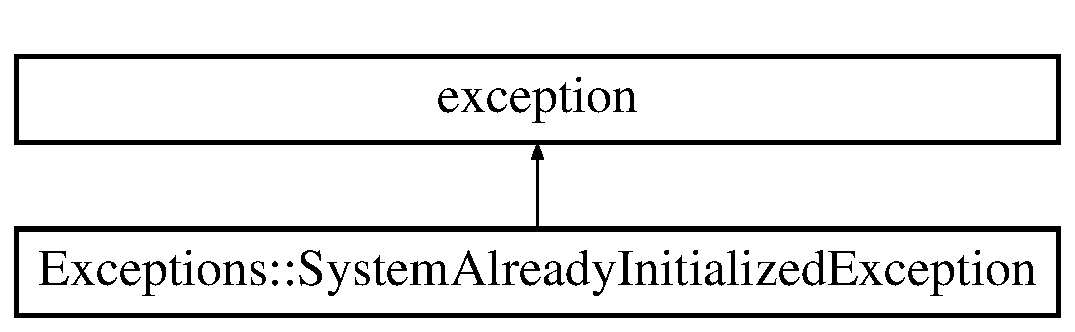
\includegraphics[height=2.000000cm]{class_exceptions_1_1_system_already_initialized_exception}
\end{center}
\end{figure}
\subsection*{Public Member Functions}
\begin{DoxyCompactItemize}
\item 
\hyperlink{class_exceptions_1_1_system_already_initialized_exception_a2f92ee1627417086ca29f3d58a8be520}{System\+Already\+Initialized\+Exception} (std\+::string \hyperlink{class_exceptions_1_1_system_already_initialized_exception_a858d81e072cf8a6a06a4fa506700fb32}{system\+\_\+name})
\item 
virtual const char $\ast$ \hyperlink{class_exceptions_1_1_system_already_initialized_exception_a28077450404b8dd5c89a348bc19ffa19}{what} () const   throw ()
\end{DoxyCompactItemize}
\subsection*{Private Attributes}
\begin{DoxyCompactItemize}
\item 
std\+::string \hyperlink{class_exceptions_1_1_system_already_initialized_exception_a858d81e072cf8a6a06a4fa506700fb32}{system\+\_\+name}
\end{DoxyCompactItemize}


\subsection{Constructor \& Destructor Documentation}
\hypertarget{class_exceptions_1_1_system_already_initialized_exception_a2f92ee1627417086ca29f3d58a8be520}{}\index{Exceptions\+::\+System\+Already\+Initialized\+Exception@{Exceptions\+::\+System\+Already\+Initialized\+Exception}!System\+Already\+Initialized\+Exception@{System\+Already\+Initialized\+Exception}}
\index{System\+Already\+Initialized\+Exception@{System\+Already\+Initialized\+Exception}!Exceptions\+::\+System\+Already\+Initialized\+Exception@{Exceptions\+::\+System\+Already\+Initialized\+Exception}}
\subsubsection[{System\+Already\+Initialized\+Exception}]{\setlength{\rightskip}{0pt plus 5cm}Exceptions\+::\+System\+Already\+Initialized\+Exception\+::\+System\+Already\+Initialized\+Exception (
\begin{DoxyParamCaption}
\item[{std\+::string}]{system\+\_\+name}
\end{DoxyParamCaption}
)\hspace{0.3cm}{\ttfamily [inline]}}\label{class_exceptions_1_1_system_already_initialized_exception_a2f92ee1627417086ca29f3d58a8be520}


\subsection{Member Function Documentation}
\hypertarget{class_exceptions_1_1_system_already_initialized_exception_a28077450404b8dd5c89a348bc19ffa19}{}\index{Exceptions\+::\+System\+Already\+Initialized\+Exception@{Exceptions\+::\+System\+Already\+Initialized\+Exception}!what@{what}}
\index{what@{what}!Exceptions\+::\+System\+Already\+Initialized\+Exception@{Exceptions\+::\+System\+Already\+Initialized\+Exception}}
\subsubsection[{what}]{\setlength{\rightskip}{0pt plus 5cm}virtual const char$\ast$ Exceptions\+::\+System\+Already\+Initialized\+Exception\+::what (
\begin{DoxyParamCaption}
{}
\end{DoxyParamCaption}
) const throw  ) \hspace{0.3cm}{\ttfamily [inline]}, {\ttfamily [virtual]}}\label{class_exceptions_1_1_system_already_initialized_exception_a28077450404b8dd5c89a348bc19ffa19}


\subsection{Member Data Documentation}
\hypertarget{class_exceptions_1_1_system_already_initialized_exception_a858d81e072cf8a6a06a4fa506700fb32}{}\index{Exceptions\+::\+System\+Already\+Initialized\+Exception@{Exceptions\+::\+System\+Already\+Initialized\+Exception}!system\+\_\+name@{system\+\_\+name}}
\index{system\+\_\+name@{system\+\_\+name}!Exceptions\+::\+System\+Already\+Initialized\+Exception@{Exceptions\+::\+System\+Already\+Initialized\+Exception}}
\subsubsection[{system\+\_\+name}]{\setlength{\rightskip}{0pt plus 5cm}std\+::string Exceptions\+::\+System\+Already\+Initialized\+Exception\+::system\+\_\+name\hspace{0.3cm}{\ttfamily [private]}}\label{class_exceptions_1_1_system_already_initialized_exception_a858d81e072cf8a6a06a4fa506700fb32}


The documentation for this class was generated from the following file\+:\begin{DoxyCompactItemize}
\item 
src/exceptions/\hyperlink{system__already__initialized__exception_8h}{system\+\_\+already\+\_\+initialized\+\_\+exception.\+h}\end{DoxyCompactItemize}

\hypertarget{class_exceptions_1_1_system_already_running_exception}{}\section{Exceptions\+:\+:System\+Already\+Running\+Exception Class Reference}
\label{class_exceptions_1_1_system_already_running_exception}\index{Exceptions\+::\+System\+Already\+Running\+Exception@{Exceptions\+::\+System\+Already\+Running\+Exception}}


{\ttfamily \#include $<$system\+\_\+already\+\_\+running\+\_\+exception.\+h$>$}

Inheritance diagram for Exceptions\+:\+:System\+Already\+Running\+Exception\+:\begin{figure}[H]
\begin{center}
\leavevmode
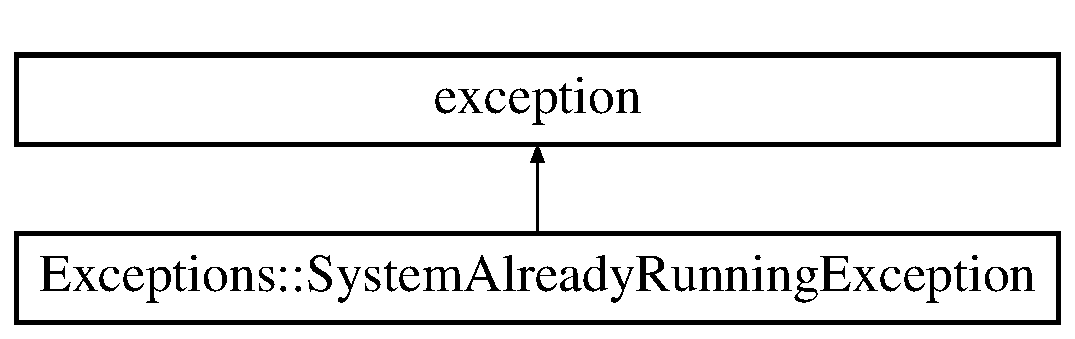
\includegraphics[height=2.000000cm]{class_exceptions_1_1_system_already_running_exception}
\end{center}
\end{figure}
\subsection*{Public Member Functions}
\begin{DoxyCompactItemize}
\item 
\hyperlink{class_exceptions_1_1_system_already_running_exception_aed8f9f444543924acea118e7485fdbba}{System\+Already\+Running\+Exception} (std\+::string \hyperlink{class_exceptions_1_1_system_already_running_exception_a914a5cb77c9acbd05862c8927da7ea36}{system\+\_\+name})
\item 
virtual const char $\ast$ \hyperlink{class_exceptions_1_1_system_already_running_exception_a558ddbeefc7c578b0a2c7ac031a5aef5}{what} () const   throw ()
\end{DoxyCompactItemize}
\subsection*{Private Attributes}
\begin{DoxyCompactItemize}
\item 
std\+::string \hyperlink{class_exceptions_1_1_system_already_running_exception_a914a5cb77c9acbd05862c8927da7ea36}{system\+\_\+name}
\end{DoxyCompactItemize}


\subsection{Constructor \& Destructor Documentation}
\hypertarget{class_exceptions_1_1_system_already_running_exception_aed8f9f444543924acea118e7485fdbba}{}\index{Exceptions\+::\+System\+Already\+Running\+Exception@{Exceptions\+::\+System\+Already\+Running\+Exception}!System\+Already\+Running\+Exception@{System\+Already\+Running\+Exception}}
\index{System\+Already\+Running\+Exception@{System\+Already\+Running\+Exception}!Exceptions\+::\+System\+Already\+Running\+Exception@{Exceptions\+::\+System\+Already\+Running\+Exception}}
\subsubsection[{System\+Already\+Running\+Exception}]{\setlength{\rightskip}{0pt plus 5cm}Exceptions\+::\+System\+Already\+Running\+Exception\+::\+System\+Already\+Running\+Exception (
\begin{DoxyParamCaption}
\item[{std\+::string}]{system\+\_\+name}
\end{DoxyParamCaption}
)\hspace{0.3cm}{\ttfamily [inline]}}\label{class_exceptions_1_1_system_already_running_exception_aed8f9f444543924acea118e7485fdbba}


\subsection{Member Function Documentation}
\hypertarget{class_exceptions_1_1_system_already_running_exception_a558ddbeefc7c578b0a2c7ac031a5aef5}{}\index{Exceptions\+::\+System\+Already\+Running\+Exception@{Exceptions\+::\+System\+Already\+Running\+Exception}!what@{what}}
\index{what@{what}!Exceptions\+::\+System\+Already\+Running\+Exception@{Exceptions\+::\+System\+Already\+Running\+Exception}}
\subsubsection[{what}]{\setlength{\rightskip}{0pt plus 5cm}virtual const char$\ast$ Exceptions\+::\+System\+Already\+Running\+Exception\+::what (
\begin{DoxyParamCaption}
{}
\end{DoxyParamCaption}
) const throw  ) \hspace{0.3cm}{\ttfamily [inline]}, {\ttfamily [virtual]}}\label{class_exceptions_1_1_system_already_running_exception_a558ddbeefc7c578b0a2c7ac031a5aef5}


\subsection{Member Data Documentation}
\hypertarget{class_exceptions_1_1_system_already_running_exception_a914a5cb77c9acbd05862c8927da7ea36}{}\index{Exceptions\+::\+System\+Already\+Running\+Exception@{Exceptions\+::\+System\+Already\+Running\+Exception}!system\+\_\+name@{system\+\_\+name}}
\index{system\+\_\+name@{system\+\_\+name}!Exceptions\+::\+System\+Already\+Running\+Exception@{Exceptions\+::\+System\+Already\+Running\+Exception}}
\subsubsection[{system\+\_\+name}]{\setlength{\rightskip}{0pt plus 5cm}std\+::string Exceptions\+::\+System\+Already\+Running\+Exception\+::system\+\_\+name\hspace{0.3cm}{\ttfamily [private]}}\label{class_exceptions_1_1_system_already_running_exception_a914a5cb77c9acbd05862c8927da7ea36}


The documentation for this class was generated from the following file\+:\begin{DoxyCompactItemize}
\item 
src/exceptions/\hyperlink{system__already__running__exception_8h}{system\+\_\+already\+\_\+running\+\_\+exception.\+h}\end{DoxyCompactItemize}

\hypertarget{class_exceptions_1_1_system_not_initialized_exception}{}\section{Exceptions\+:\+:System\+Not\+Initialized\+Exception Class Reference}
\label{class_exceptions_1_1_system_not_initialized_exception}\index{Exceptions\+::\+System\+Not\+Initialized\+Exception@{Exceptions\+::\+System\+Not\+Initialized\+Exception}}


{\ttfamily \#include $<$system\+\_\+not\+\_\+initialized\+\_\+exception.\+h$>$}

Inheritance diagram for Exceptions\+:\+:System\+Not\+Initialized\+Exception\+:\begin{figure}[H]
\begin{center}
\leavevmode
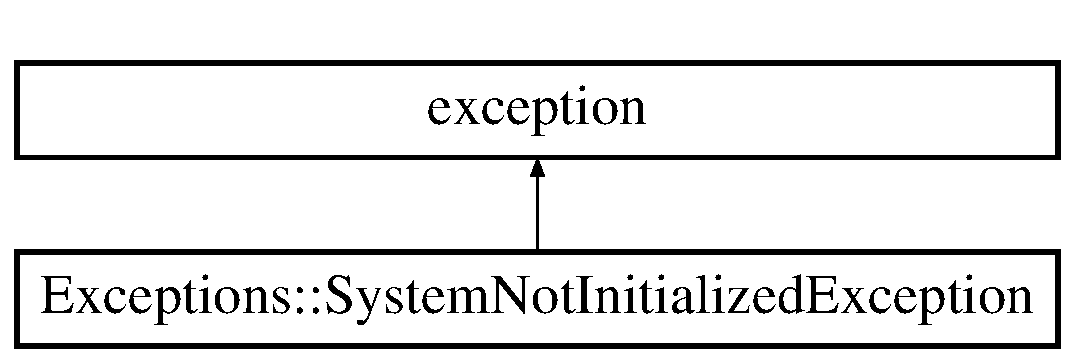
\includegraphics[height=2.000000cm]{class_exceptions_1_1_system_not_initialized_exception}
\end{center}
\end{figure}
\subsection*{Public Member Functions}
\begin{DoxyCompactItemize}
\item 
\hyperlink{class_exceptions_1_1_system_not_initialized_exception_ac22625946ad8f784f8c78b1b5b2970d7}{System\+Not\+Initialized\+Exception} (std\+::string \hyperlink{class_exceptions_1_1_system_not_initialized_exception_a5649bbb869394d52f7c8aa82d600d070}{system\+\_\+name})
\item 
virtual const char $\ast$ \hyperlink{class_exceptions_1_1_system_not_initialized_exception_a6481e3f2f2dd245e47ed246b12ce61c5}{what} () const   throw ()
\end{DoxyCompactItemize}
\subsection*{Private Attributes}
\begin{DoxyCompactItemize}
\item 
std\+::string \hyperlink{class_exceptions_1_1_system_not_initialized_exception_a5649bbb869394d52f7c8aa82d600d070}{system\+\_\+name}
\end{DoxyCompactItemize}


\subsection{Constructor \& Destructor Documentation}
\hypertarget{class_exceptions_1_1_system_not_initialized_exception_ac22625946ad8f784f8c78b1b5b2970d7}{}\index{Exceptions\+::\+System\+Not\+Initialized\+Exception@{Exceptions\+::\+System\+Not\+Initialized\+Exception}!System\+Not\+Initialized\+Exception@{System\+Not\+Initialized\+Exception}}
\index{System\+Not\+Initialized\+Exception@{System\+Not\+Initialized\+Exception}!Exceptions\+::\+System\+Not\+Initialized\+Exception@{Exceptions\+::\+System\+Not\+Initialized\+Exception}}
\subsubsection[{System\+Not\+Initialized\+Exception}]{\setlength{\rightskip}{0pt plus 5cm}Exceptions\+::\+System\+Not\+Initialized\+Exception\+::\+System\+Not\+Initialized\+Exception (
\begin{DoxyParamCaption}
\item[{std\+::string}]{system\+\_\+name}
\end{DoxyParamCaption}
)\hspace{0.3cm}{\ttfamily [inline]}}\label{class_exceptions_1_1_system_not_initialized_exception_ac22625946ad8f784f8c78b1b5b2970d7}


\subsection{Member Function Documentation}
\hypertarget{class_exceptions_1_1_system_not_initialized_exception_a6481e3f2f2dd245e47ed246b12ce61c5}{}\index{Exceptions\+::\+System\+Not\+Initialized\+Exception@{Exceptions\+::\+System\+Not\+Initialized\+Exception}!what@{what}}
\index{what@{what}!Exceptions\+::\+System\+Not\+Initialized\+Exception@{Exceptions\+::\+System\+Not\+Initialized\+Exception}}
\subsubsection[{what}]{\setlength{\rightskip}{0pt plus 5cm}virtual const char$\ast$ Exceptions\+::\+System\+Not\+Initialized\+Exception\+::what (
\begin{DoxyParamCaption}
{}
\end{DoxyParamCaption}
) const throw  ) \hspace{0.3cm}{\ttfamily [inline]}, {\ttfamily [virtual]}}\label{class_exceptions_1_1_system_not_initialized_exception_a6481e3f2f2dd245e47ed246b12ce61c5}


\subsection{Member Data Documentation}
\hypertarget{class_exceptions_1_1_system_not_initialized_exception_a5649bbb869394d52f7c8aa82d600d070}{}\index{Exceptions\+::\+System\+Not\+Initialized\+Exception@{Exceptions\+::\+System\+Not\+Initialized\+Exception}!system\+\_\+name@{system\+\_\+name}}
\index{system\+\_\+name@{system\+\_\+name}!Exceptions\+::\+System\+Not\+Initialized\+Exception@{Exceptions\+::\+System\+Not\+Initialized\+Exception}}
\subsubsection[{system\+\_\+name}]{\setlength{\rightskip}{0pt plus 5cm}std\+::string Exceptions\+::\+System\+Not\+Initialized\+Exception\+::system\+\_\+name\hspace{0.3cm}{\ttfamily [private]}}\label{class_exceptions_1_1_system_not_initialized_exception_a5649bbb869394d52f7c8aa82d600d070}


The documentation for this class was generated from the following file\+:\begin{DoxyCompactItemize}
\item 
src/exceptions/\hyperlink{system__not__initialized__exception_8h}{system\+\_\+not\+\_\+initialized\+\_\+exception.\+h}\end{DoxyCompactItemize}

\hypertarget{class_exceptions_1_1_system_not_running_exception}{}\section{Exceptions\+:\+:System\+Not\+Running\+Exception Class Reference}
\label{class_exceptions_1_1_system_not_running_exception}\index{Exceptions\+::\+System\+Not\+Running\+Exception@{Exceptions\+::\+System\+Not\+Running\+Exception}}


{\ttfamily \#include $<$system\+\_\+not\+\_\+running\+\_\+exception.\+h$>$}

Inheritance diagram for Exceptions\+:\+:System\+Not\+Running\+Exception\+:\begin{figure}[H]
\begin{center}
\leavevmode
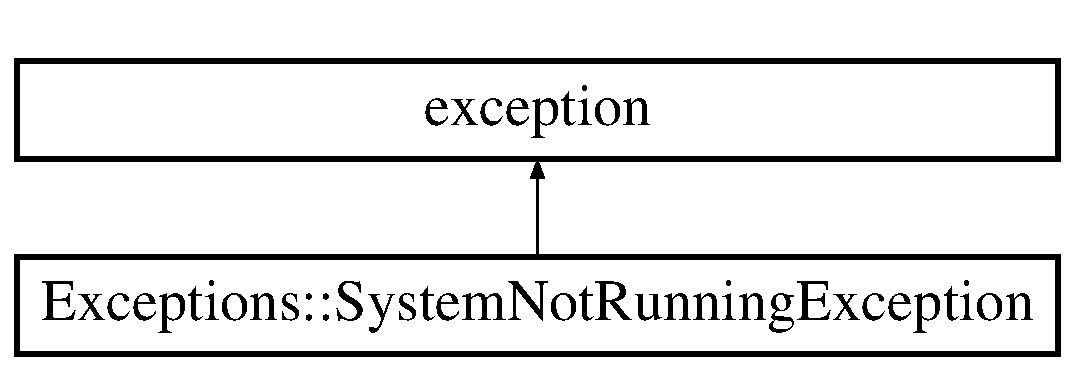
\includegraphics[height=2.000000cm]{class_exceptions_1_1_system_not_running_exception}
\end{center}
\end{figure}
\subsection*{Public Member Functions}
\begin{DoxyCompactItemize}
\item 
\hyperlink{class_exceptions_1_1_system_not_running_exception_aed32e775ba2eb68ff70446c138c40bcc}{System\+Not\+Running\+Exception} (std\+::string \hyperlink{class_exceptions_1_1_system_not_running_exception_af97cd0ba9e5c5b4aa57b99028b6bb95a}{system\+\_\+name})
\item 
virtual const char $\ast$ \hyperlink{class_exceptions_1_1_system_not_running_exception_afc7a24ce91303377321104405996f5ff}{what} () const   throw ()
\end{DoxyCompactItemize}
\subsection*{Private Attributes}
\begin{DoxyCompactItemize}
\item 
std\+::string \hyperlink{class_exceptions_1_1_system_not_running_exception_af97cd0ba9e5c5b4aa57b99028b6bb95a}{system\+\_\+name}
\end{DoxyCompactItemize}


\subsection{Constructor \& Destructor Documentation}
\hypertarget{class_exceptions_1_1_system_not_running_exception_aed32e775ba2eb68ff70446c138c40bcc}{}\index{Exceptions\+::\+System\+Not\+Running\+Exception@{Exceptions\+::\+System\+Not\+Running\+Exception}!System\+Not\+Running\+Exception@{System\+Not\+Running\+Exception}}
\index{System\+Not\+Running\+Exception@{System\+Not\+Running\+Exception}!Exceptions\+::\+System\+Not\+Running\+Exception@{Exceptions\+::\+System\+Not\+Running\+Exception}}
\subsubsection[{System\+Not\+Running\+Exception}]{\setlength{\rightskip}{0pt plus 5cm}Exceptions\+::\+System\+Not\+Running\+Exception\+::\+System\+Not\+Running\+Exception (
\begin{DoxyParamCaption}
\item[{std\+::string}]{system\+\_\+name}
\end{DoxyParamCaption}
)\hspace{0.3cm}{\ttfamily [inline]}}\label{class_exceptions_1_1_system_not_running_exception_aed32e775ba2eb68ff70446c138c40bcc}


\subsection{Member Function Documentation}
\hypertarget{class_exceptions_1_1_system_not_running_exception_afc7a24ce91303377321104405996f5ff}{}\index{Exceptions\+::\+System\+Not\+Running\+Exception@{Exceptions\+::\+System\+Not\+Running\+Exception}!what@{what}}
\index{what@{what}!Exceptions\+::\+System\+Not\+Running\+Exception@{Exceptions\+::\+System\+Not\+Running\+Exception}}
\subsubsection[{what}]{\setlength{\rightskip}{0pt plus 5cm}virtual const char$\ast$ Exceptions\+::\+System\+Not\+Running\+Exception\+::what (
\begin{DoxyParamCaption}
{}
\end{DoxyParamCaption}
) const throw  ) \hspace{0.3cm}{\ttfamily [inline]}, {\ttfamily [virtual]}}\label{class_exceptions_1_1_system_not_running_exception_afc7a24ce91303377321104405996f5ff}


\subsection{Member Data Documentation}
\hypertarget{class_exceptions_1_1_system_not_running_exception_af97cd0ba9e5c5b4aa57b99028b6bb95a}{}\index{Exceptions\+::\+System\+Not\+Running\+Exception@{Exceptions\+::\+System\+Not\+Running\+Exception}!system\+\_\+name@{system\+\_\+name}}
\index{system\+\_\+name@{system\+\_\+name}!Exceptions\+::\+System\+Not\+Running\+Exception@{Exceptions\+::\+System\+Not\+Running\+Exception}}
\subsubsection[{system\+\_\+name}]{\setlength{\rightskip}{0pt plus 5cm}std\+::string Exceptions\+::\+System\+Not\+Running\+Exception\+::system\+\_\+name\hspace{0.3cm}{\ttfamily [private]}}\label{class_exceptions_1_1_system_not_running_exception_af97cd0ba9e5c5b4aa57b99028b6bb95a}


The documentation for this class was generated from the following file\+:\begin{DoxyCompactItemize}
\item 
src/exceptions/\hyperlink{system__not__running__exception_8h}{system\+\_\+not\+\_\+running\+\_\+exception.\+h}\end{DoxyCompactItemize}

\chapter{File Documentation}
\hypertarget{system__already__initialized__exception_8h}{}\section{src/exceptions/system\+\_\+already\+\_\+initialized\+\_\+exception.h File Reference}
\label{system__already__initialized__exception_8h}\index{src/exceptions/system\+\_\+already\+\_\+initialized\+\_\+exception.\+h@{src/exceptions/system\+\_\+already\+\_\+initialized\+\_\+exception.\+h}}
{\ttfamily \#include $<$exception$>$}\\*
\subsection*{Classes}
\begin{DoxyCompactItemize}
\item 
class \hyperlink{class_exceptions_1_1_system_already_initialized_exception}{Exceptions\+::\+System\+Already\+Initialized\+Exception}
\end{DoxyCompactItemize}
\subsection*{Namespaces}
\begin{DoxyCompactItemize}
\item 
 \hyperlink{namespace_exceptions}{Exceptions}
\end{DoxyCompactItemize}

\hypertarget{system__already__running__exception_8h}{}\section{src/exceptions/system\+\_\+already\+\_\+running\+\_\+exception.h File Reference}
\label{system__already__running__exception_8h}\index{src/exceptions/system\+\_\+already\+\_\+running\+\_\+exception.\+h@{src/exceptions/system\+\_\+already\+\_\+running\+\_\+exception.\+h}}
{\ttfamily \#include $<$exception$>$}\\*
\subsection*{Classes}
\begin{DoxyCompactItemize}
\item 
class \hyperlink{class_exceptions_1_1_system_already_running_exception}{Exceptions\+::\+System\+Already\+Running\+Exception}
\end{DoxyCompactItemize}
\subsection*{Namespaces}
\begin{DoxyCompactItemize}
\item 
 \hyperlink{namespace_exceptions}{Exceptions}
\end{DoxyCompactItemize}

\hypertarget{system__not__initialized__exception_8h}{}\section{src/exceptions/system\+\_\+not\+\_\+initialized\+\_\+exception.h File Reference}
\label{system__not__initialized__exception_8h}\index{src/exceptions/system\+\_\+not\+\_\+initialized\+\_\+exception.\+h@{src/exceptions/system\+\_\+not\+\_\+initialized\+\_\+exception.\+h}}
{\ttfamily \#include $<$exception$>$}\\*
\subsection*{Classes}
\begin{DoxyCompactItemize}
\item 
class \hyperlink{class_exceptions_1_1_system_not_initialized_exception}{Exceptions\+::\+System\+Not\+Initialized\+Exception}
\end{DoxyCompactItemize}
\subsection*{Namespaces}
\begin{DoxyCompactItemize}
\item 
 \hyperlink{namespace_exceptions}{Exceptions}
\end{DoxyCompactItemize}

\hypertarget{system__not__running__exception_8h}{}\section{src/exceptions/system\+\_\+not\+\_\+running\+\_\+exception.h File Reference}
\label{system__not__running__exception_8h}\index{src/exceptions/system\+\_\+not\+\_\+running\+\_\+exception.\+h@{src/exceptions/system\+\_\+not\+\_\+running\+\_\+exception.\+h}}
{\ttfamily \#include $<$exception$>$}\\*
\subsection*{Classes}
\begin{DoxyCompactItemize}
\item 
class \hyperlink{class_exceptions_1_1_system_not_running_exception}{Exceptions\+::\+System\+Not\+Running\+Exception}
\end{DoxyCompactItemize}
\subsection*{Namespaces}
\begin{DoxyCompactItemize}
\item 
 \hyperlink{namespace_exceptions}{Exceptions}
\end{DoxyCompactItemize}

\hypertarget{graphics__system_8cpp}{}\section{src/graphics/graphics\+\_\+system.cpp File Reference}
\label{graphics__system_8cpp}\index{src/graphics/graphics\+\_\+system.\+cpp@{src/graphics/graphics\+\_\+system.\+cpp}}
{\ttfamily \#include $<$easylogging++.\+h$>$}\\*
{\ttfamily \#include \char`\"{}graphics\+\_\+system.\+h\char`\"{}}\\*
{\ttfamily \#include $<$exception$>$}\\*
{\ttfamily \#include $<$stdexcept$>$}\\*
{\ttfamily \#include $<$system\+\_\+error$>$}\\*
{\ttfamily \#include \char`\"{}exceptions/system\+\_\+already\+\_\+initialized\+\_\+exception.\+h\char`\"{}}\\*
{\ttfamily \#include \char`\"{}exceptions/system\+\_\+not\+\_\+initialized\+\_\+exception.\+h\char`\"{}}\\*
{\ttfamily \#include \char`\"{}exceptions/system\+\_\+already\+\_\+running\+\_\+exception.\+h\char`\"{}}\\*
{\ttfamily \#include \char`\"{}exceptions/system\+\_\+not\+\_\+running\+\_\+exception.\+h\char`\"{}}\\*
\subsection*{Namespaces}
\begin{DoxyCompactItemize}
\item 
 \hyperlink{namespace_graphics}{Graphics}
\end{DoxyCompactItemize}

\hypertarget{graphics__system_8h}{}\section{src/graphics/graphics\+\_\+system.h File Reference}
\label{graphics__system_8h}\index{src/graphics/graphics\+\_\+system.\+h@{src/graphics/graphics\+\_\+system.\+h}}
{\ttfamily \#include $<$thread$>$}\\*
{\ttfamily \#include $<$atomic$>$}\\*
{\ttfamily \#include $<$map$>$}\\*
{\ttfamily \#include $<$set$>$}\\*
{\ttfamily \#include $<$chrono$>$}\\*
{\ttfamily \#include $<$mutex$>$}\\*
{\ttfamily \#include $<$glfw3.\+h$>$}\\*
{\ttfamily \#include \char`\"{}graphics/renderable.\+h\char`\"{}}\\*
{\ttfamily \#include \char`\"{}graphics/window\+\_\+exit\+\_\+functor.\+h\char`\"{}}\\*
\subsection*{Classes}
\begin{DoxyCompactItemize}
\item 
class \hyperlink{class_graphics_1_1_graphics_system}{Graphics\+::\+Graphics\+System}
\end{DoxyCompactItemize}
\subsection*{Namespaces}
\begin{DoxyCompactItemize}
\item 
 \hyperlink{namespace_graphics}{Graphics}
\end{DoxyCompactItemize}

\hypertarget{main_8cpp}{}\section{src/main.cpp File Reference}
\label{main_8cpp}\index{src/main.\+cpp@{src/main.\+cpp}}
{\ttfamily \#include $<$easylogging++.\+h$>$}\\*
{\ttfamily \#include $<$iostream$>$}\\*
{\ttfamily \#include $<$glm/vec3.\+hpp$>$}\\*
{\ttfamily \#include $<$Open\+G\+L/gl3.\+h$>$}\\*
{\ttfamily \#include $<$glfw3.\+h$>$}\\*
{\ttfamily \#include \char`\"{}graphics/graphics\+\_\+system.\+h\char`\"{}}\\*
{\ttfamily \#include \char`\"{}graphics/renderable.\+h\char`\"{}}\\*
{\ttfamily \#include \char`\"{}graphics/vertex\+\_\+data.\+h\char`\"{}}\\*
{\ttfamily \#include \char`\"{}graphics/window\+\_\+exit\+\_\+functor.\+h\char`\"{}}\\*
{\ttfamily \#include \char`\"{}graphics/tile\+\_\+attribute\+\_\+trait.\+h\char`\"{}}\\*
{\ttfamily \#include \char`\"{}graphics/shader.\+h\char`\"{}}\\*
\subsection*{Macros}
\begin{DoxyCompactItemize}
\item 
\#define \hyperlink{main_8cpp_a2e25352eed9ac9fe7758aaf000575577}{E\+L\+P\+P\+\_\+\+T\+H\+R\+E\+A\+D\+\_\+\+S\+A\+F\+E}
\end{DoxyCompactItemize}
\subsection*{Functions}
\begin{DoxyCompactItemize}
\item 
unsigned int \hyperlink{main_8cpp_aeacc9dbd3a3374fd4e0856a3ecf7224d}{generate\+\_\+valid\+\_\+fragment} ()
\item 
unsigned int \hyperlink{main_8cpp_a17049b22143dc4bbb930c2263ff88541}{generate\+\_\+valid\+\_\+vertex} ()
\item 
int \hyperlink{main_8cpp_a3c04138a5bfe5d72780bb7e82a18e627}{main} (int argc, char $\ast$$\ast$argv)
\end{DoxyCompactItemize}


\subsection{Macro Definition Documentation}
\hypertarget{main_8cpp_a2e25352eed9ac9fe7758aaf000575577}{}\index{main.\+cpp@{main.\+cpp}!E\+L\+P\+P\+\_\+\+T\+H\+R\+E\+A\+D\+\_\+\+S\+A\+F\+E@{E\+L\+P\+P\+\_\+\+T\+H\+R\+E\+A\+D\+\_\+\+S\+A\+F\+E}}
\index{E\+L\+P\+P\+\_\+\+T\+H\+R\+E\+A\+D\+\_\+\+S\+A\+F\+E@{E\+L\+P\+P\+\_\+\+T\+H\+R\+E\+A\+D\+\_\+\+S\+A\+F\+E}!main.\+cpp@{main.\+cpp}}
\subsubsection[{E\+L\+P\+P\+\_\+\+T\+H\+R\+E\+A\+D\+\_\+\+S\+A\+F\+E}]{\setlength{\rightskip}{0pt plus 5cm}\#define E\+L\+P\+P\+\_\+\+T\+H\+R\+E\+A\+D\+\_\+\+S\+A\+F\+E}\label{main_8cpp_a2e25352eed9ac9fe7758aaf000575577}


\subsection{Function Documentation}
\hypertarget{main_8cpp_aeacc9dbd3a3374fd4e0856a3ecf7224d}{}\index{main.\+cpp@{main.\+cpp}!generate\+\_\+valid\+\_\+fragment@{generate\+\_\+valid\+\_\+fragment}}
\index{generate\+\_\+valid\+\_\+fragment@{generate\+\_\+valid\+\_\+fragment}!main.\+cpp@{main.\+cpp}}
\subsubsection[{generate\+\_\+valid\+\_\+fragment}]{\setlength{\rightskip}{0pt plus 5cm}unsigned int generate\+\_\+valid\+\_\+fragment (
\begin{DoxyParamCaption}
{}
\end{DoxyParamCaption}
)}\label{main_8cpp_aeacc9dbd3a3374fd4e0856a3ecf7224d}
\hypertarget{main_8cpp_a17049b22143dc4bbb930c2263ff88541}{}\index{main.\+cpp@{main.\+cpp}!generate\+\_\+valid\+\_\+vertex@{generate\+\_\+valid\+\_\+vertex}}
\index{generate\+\_\+valid\+\_\+vertex@{generate\+\_\+valid\+\_\+vertex}!main.\+cpp@{main.\+cpp}}
\subsubsection[{generate\+\_\+valid\+\_\+vertex}]{\setlength{\rightskip}{0pt plus 5cm}unsigned int generate\+\_\+valid\+\_\+vertex (
\begin{DoxyParamCaption}
{}
\end{DoxyParamCaption}
)}\label{main_8cpp_a17049b22143dc4bbb930c2263ff88541}
\hypertarget{main_8cpp_a3c04138a5bfe5d72780bb7e82a18e627}{}\index{main.\+cpp@{main.\+cpp}!main@{main}}
\index{main@{main}!main.\+cpp@{main.\+cpp}}
\subsubsection[{main}]{\setlength{\rightskip}{0pt plus 5cm}int main (
\begin{DoxyParamCaption}
\item[{int}]{argc, }
\item[{char $\ast$$\ast$}]{argv}
\end{DoxyParamCaption}
)}\label{main_8cpp_a3c04138a5bfe5d72780bb7e82a18e627}

\hypertarget{graphics__system__test_8cpp}{}\section{test/graphics/graphics\+\_\+system\+\_\+test.cpp File Reference}
\label{graphics__system__test_8cpp}\index{test/graphics/graphics\+\_\+system\+\_\+test.\+cpp@{test/graphics/graphics\+\_\+system\+\_\+test.\+cpp}}
{\ttfamily \#include $<$easylogging++.\+h$>$}\\*
{\ttfamily \#include $<$catch.\+hpp$>$}\\*
{\ttfamily \#include $<$iostream$>$}\\*
{\ttfamily \#include $<$random$>$}\\*
{\ttfamily \#include $<$thread$>$}\\*
{\ttfamily \#include $<$memory$>$}\\*
{\ttfamily \#include $<$Open\+G\+L/gl3.\+h$>$}\\*
{\ttfamily \#include $<$glfw3.\+h$>$}\\*
{\ttfamily \#include \char`\"{}graphics/graphics\+\_\+system.\+h\char`\"{}}\\*
{\ttfamily \#include \char`\"{}graphics/renderable.\+h\char`\"{}}\\*
{\ttfamily \#include \char`\"{}graphics/vertex\+\_\+data.\+h\char`\"{}}\\*
{\ttfamily \#include \char`\"{}graphics/window\+\_\+exit\+\_\+functor.\+h\char`\"{}}\\*
{\ttfamily \#include \char`\"{}graphics/tile\+\_\+attribute\+\_\+trait.\+h\char`\"{}}\\*
{\ttfamily \#include \char`\"{}exceptions/system\+\_\+already\+\_\+initialized\+\_\+exception.\+h\char`\"{}}\\*
{\ttfamily \#include \char`\"{}exceptions/system\+\_\+not\+\_\+initialized\+\_\+exception.\+h\char`\"{}}\\*
{\ttfamily \#include \char`\"{}exceptions/system\+\_\+already\+\_\+running\+\_\+exception.\+h\char`\"{}}\\*
{\ttfamily \#include \char`\"{}exceptions/system\+\_\+not\+\_\+running\+\_\+exception.\+h\char`\"{}}\\*
{\ttfamily \#include \char`\"{}exceptions/invalid\+\_\+vertex\+\_\+array\+\_\+exception.\+h\char`\"{}}\\*
\subsection*{Typedefs}
\begin{DoxyCompactItemize}
\item 
using \hyperlink{graphics__system__test_8cpp_abf7941403e8dd3db88bd66f0d775555a}{Renderable\+Ptr} = std\+::shared\+\_\+ptr$<$ \hyperlink{class_graphics_1_1_renderable}{Graphics\+::\+Renderable} $>$
\end{DoxyCompactItemize}
\subsection*{Functions}
\begin{DoxyCompactItemize}
\item 
\hyperlink{graphics__system__test_8cpp_abf7941403e8dd3db88bd66f0d775555a}{Renderable\+Ptr} \hyperlink{graphics__system__test_8cpp_afeb3ce1ce648dadcf4c64857a658a388}{construct\+Renderable} ()
\item 
\hyperlink{graphics__system__test_8cpp_acb8214ec493a3617eff027e38c555270}{S\+C\+E\+N\+A\+R\+I\+O} (\char`\"{}the graphics system can be initialized\char`\"{},\char`\"{}\mbox{[}graphics\mbox{]}\char`\"{})
\item 
\hyperlink{graphics__system__test_8cpp_ac224d651330e1a5717d34b10b27ad273}{S\+C\+E\+N\+A\+R\+I\+O} (\char`\"{}the graphics system can be destroyed\char`\"{},\char`\"{}\mbox{[}graphics\mbox{]}\char`\"{})
\item 
\hyperlink{graphics__system__test_8cpp_ac2199b10682bd556118f1ae71ce7c743}{S\+C\+E\+N\+A\+R\+I\+O} (\char`\"{}the graphics system can have objects for rendering added to it\char`\"{},\char`\"{}\mbox{[}graphics\mbox{]}\char`\"{})
\item 
\hyperlink{graphics__system__test_8cpp_a3ca4ab95742c1cb589848e6590f5a07f}{S\+C\+E\+N\+A\+R\+I\+O} (\char`\"{}the graphics system can have objects for rendering removed from it\char`\"{},\char`\"{}\mbox{[}graphics\mbox{]}\char`\"{})
\item 
\hyperlink{graphics__system__test_8cpp_a7e4a8d64e1fca8af44728f0e3c6a5d59}{S\+C\+E\+N\+A\+R\+I\+O} (\char`\"{}the window\textquotesingle{}s width and height can be retrieved\char`\"{})
\end{DoxyCompactItemize}


\subsection{Typedef Documentation}
\hypertarget{graphics__system__test_8cpp_abf7941403e8dd3db88bd66f0d775555a}{}\index{graphics\+\_\+system\+\_\+test.\+cpp@{graphics\+\_\+system\+\_\+test.\+cpp}!Renderable\+Ptr@{Renderable\+Ptr}}
\index{Renderable\+Ptr@{Renderable\+Ptr}!graphics\+\_\+system\+\_\+test.\+cpp@{graphics\+\_\+system\+\_\+test.\+cpp}}
\subsubsection[{Renderable\+Ptr}]{\setlength{\rightskip}{0pt plus 5cm}using {\bf Renderable\+Ptr} =  std\+::shared\+\_\+ptr$<${\bf Graphics\+::\+Renderable}$>$}\label{graphics__system__test_8cpp_abf7941403e8dd3db88bd66f0d775555a}


\subsection{Function Documentation}
\hypertarget{graphics__system__test_8cpp_afeb3ce1ce648dadcf4c64857a658a388}{}\index{graphics\+\_\+system\+\_\+test.\+cpp@{graphics\+\_\+system\+\_\+test.\+cpp}!construct\+Renderable@{construct\+Renderable}}
\index{construct\+Renderable@{construct\+Renderable}!graphics\+\_\+system\+\_\+test.\+cpp@{graphics\+\_\+system\+\_\+test.\+cpp}}
\subsubsection[{construct\+Renderable}]{\setlength{\rightskip}{0pt plus 5cm}{\bf Renderable\+Ptr} construct\+Renderable (
\begin{DoxyParamCaption}
{}
\end{DoxyParamCaption}
)}\label{graphics__system__test_8cpp_afeb3ce1ce648dadcf4c64857a658a388}
\hypertarget{graphics__system__test_8cpp_acb8214ec493a3617eff027e38c555270}{}\index{graphics\+\_\+system\+\_\+test.\+cpp@{graphics\+\_\+system\+\_\+test.\+cpp}!S\+C\+E\+N\+A\+R\+I\+O@{S\+C\+E\+N\+A\+R\+I\+O}}
\index{S\+C\+E\+N\+A\+R\+I\+O@{S\+C\+E\+N\+A\+R\+I\+O}!graphics\+\_\+system\+\_\+test.\+cpp@{graphics\+\_\+system\+\_\+test.\+cpp}}
\subsubsection[{S\+C\+E\+N\+A\+R\+I\+O}]{\setlength{\rightskip}{0pt plus 5cm}S\+C\+E\+N\+A\+R\+I\+O (
\begin{DoxyParamCaption}
\item[{\char`\"{}the graphics system can be initialized\char`\"{}}]{, }
\item[{\char`\"{}\char`\"{}}]{\mbox{[}graphics\mbox{]}}
\end{DoxyParamCaption}
)}\label{graphics__system__test_8cpp_acb8214ec493a3617eff027e38c555270}
\hypertarget{graphics__system__test_8cpp_ac224d651330e1a5717d34b10b27ad273}{}\index{graphics\+\_\+system\+\_\+test.\+cpp@{graphics\+\_\+system\+\_\+test.\+cpp}!S\+C\+E\+N\+A\+R\+I\+O@{S\+C\+E\+N\+A\+R\+I\+O}}
\index{S\+C\+E\+N\+A\+R\+I\+O@{S\+C\+E\+N\+A\+R\+I\+O}!graphics\+\_\+system\+\_\+test.\+cpp@{graphics\+\_\+system\+\_\+test.\+cpp}}
\subsubsection[{S\+C\+E\+N\+A\+R\+I\+O}]{\setlength{\rightskip}{0pt plus 5cm}S\+C\+E\+N\+A\+R\+I\+O (
\begin{DoxyParamCaption}
\item[{\char`\"{}the graphics system can be destroyed\char`\"{}}]{, }
\item[{\char`\"{}\char`\"{}}]{\mbox{[}graphics\mbox{]}}
\end{DoxyParamCaption}
)}\label{graphics__system__test_8cpp_ac224d651330e1a5717d34b10b27ad273}
\hypertarget{graphics__system__test_8cpp_ac2199b10682bd556118f1ae71ce7c743}{}\index{graphics\+\_\+system\+\_\+test.\+cpp@{graphics\+\_\+system\+\_\+test.\+cpp}!S\+C\+E\+N\+A\+R\+I\+O@{S\+C\+E\+N\+A\+R\+I\+O}}
\index{S\+C\+E\+N\+A\+R\+I\+O@{S\+C\+E\+N\+A\+R\+I\+O}!graphics\+\_\+system\+\_\+test.\+cpp@{graphics\+\_\+system\+\_\+test.\+cpp}}
\subsubsection[{S\+C\+E\+N\+A\+R\+I\+O}]{\setlength{\rightskip}{0pt plus 5cm}S\+C\+E\+N\+A\+R\+I\+O (
\begin{DoxyParamCaption}
\item[{\char`\"{}the graphics system can have objects for rendering added to it\char`\"{}}]{, }
\item[{\char`\"{}\char`\"{}}]{\mbox{[}graphics\mbox{]}}
\end{DoxyParamCaption}
)}\label{graphics__system__test_8cpp_ac2199b10682bd556118f1ae71ce7c743}
\hypertarget{graphics__system__test_8cpp_a3ca4ab95742c1cb589848e6590f5a07f}{}\index{graphics\+\_\+system\+\_\+test.\+cpp@{graphics\+\_\+system\+\_\+test.\+cpp}!S\+C\+E\+N\+A\+R\+I\+O@{S\+C\+E\+N\+A\+R\+I\+O}}
\index{S\+C\+E\+N\+A\+R\+I\+O@{S\+C\+E\+N\+A\+R\+I\+O}!graphics\+\_\+system\+\_\+test.\+cpp@{graphics\+\_\+system\+\_\+test.\+cpp}}
\subsubsection[{S\+C\+E\+N\+A\+R\+I\+O}]{\setlength{\rightskip}{0pt plus 5cm}S\+C\+E\+N\+A\+R\+I\+O (
\begin{DoxyParamCaption}
\item[{\char`\"{}the graphics system can have objects for rendering removed from it\char`\"{}}]{, }
\item[{\char`\"{}\char`\"{}}]{\mbox{[}graphics\mbox{]}}
\end{DoxyParamCaption}
)}\label{graphics__system__test_8cpp_a3ca4ab95742c1cb589848e6590f5a07f}
\hypertarget{graphics__system__test_8cpp_a7e4a8d64e1fca8af44728f0e3c6a5d59}{}\index{graphics\+\_\+system\+\_\+test.\+cpp@{graphics\+\_\+system\+\_\+test.\+cpp}!S\+C\+E\+N\+A\+R\+I\+O@{S\+C\+E\+N\+A\+R\+I\+O}}
\index{S\+C\+E\+N\+A\+R\+I\+O@{S\+C\+E\+N\+A\+R\+I\+O}!graphics\+\_\+system\+\_\+test.\+cpp@{graphics\+\_\+system\+\_\+test.\+cpp}}
\subsubsection[{S\+C\+E\+N\+A\+R\+I\+O}]{\setlength{\rightskip}{0pt plus 5cm}S\+C\+E\+N\+A\+R\+I\+O (
\begin{DoxyParamCaption}
\item[{\char`\"{}the window\textquotesingle{}s width and height can be retrieved\char`\"{}}]{}
\end{DoxyParamCaption}
)}\label{graphics__system__test_8cpp_a7e4a8d64e1fca8af44728f0e3c6a5d59}

\hypertarget{test__main_8cpp}{}\section{test/test\+\_\+main.cpp File Reference}
\label{test__main_8cpp}\index{test/test\+\_\+main.\+cpp@{test/test\+\_\+main.\+cpp}}
{\ttfamily \#include $<$catch.\+hpp$>$}\\*
{\ttfamily \#include $<$easylogging++.\+h$>$}\\*
\subsection*{Macros}
\begin{DoxyCompactItemize}
\item 
\#define \hyperlink{test__main_8cpp_a34b4c3eca7342fbc4cba090d02139902}{C\+A\+T\+C\+H\+\_\+\+C\+O\+N\+F\+I\+G\+\_\+\+R\+U\+N\+N\+E\+R}
\item 
\#define \hyperlink{test__main_8cpp_a2e25352eed9ac9fe7758aaf000575577}{E\+L\+P\+P\+\_\+\+T\+H\+R\+E\+A\+D\+\_\+\+S\+A\+F\+E}
\end{DoxyCompactItemize}
\subsection*{Functions}
\begin{DoxyCompactItemize}
\item 
int \hyperlink{test__main_8cpp_a3c04138a5bfe5d72780bb7e82a18e627}{main} (int argc, char $\ast$$\ast$argv)
\end{DoxyCompactItemize}


\subsection{Macro Definition Documentation}
\hypertarget{test__main_8cpp_a34b4c3eca7342fbc4cba090d02139902}{}\index{test\+\_\+main.\+cpp@{test\+\_\+main.\+cpp}!C\+A\+T\+C\+H\+\_\+\+C\+O\+N\+F\+I\+G\+\_\+\+R\+U\+N\+N\+E\+R@{C\+A\+T\+C\+H\+\_\+\+C\+O\+N\+F\+I\+G\+\_\+\+R\+U\+N\+N\+E\+R}}
\index{C\+A\+T\+C\+H\+\_\+\+C\+O\+N\+F\+I\+G\+\_\+\+R\+U\+N\+N\+E\+R@{C\+A\+T\+C\+H\+\_\+\+C\+O\+N\+F\+I\+G\+\_\+\+R\+U\+N\+N\+E\+R}!test\+\_\+main.\+cpp@{test\+\_\+main.\+cpp}}
\subsubsection[{C\+A\+T\+C\+H\+\_\+\+C\+O\+N\+F\+I\+G\+\_\+\+R\+U\+N\+N\+E\+R}]{\setlength{\rightskip}{0pt plus 5cm}\#define C\+A\+T\+C\+H\+\_\+\+C\+O\+N\+F\+I\+G\+\_\+\+R\+U\+N\+N\+E\+R}\label{test__main_8cpp_a34b4c3eca7342fbc4cba090d02139902}
\hypertarget{test__main_8cpp_a2e25352eed9ac9fe7758aaf000575577}{}\index{test\+\_\+main.\+cpp@{test\+\_\+main.\+cpp}!E\+L\+P\+P\+\_\+\+T\+H\+R\+E\+A\+D\+\_\+\+S\+A\+F\+E@{E\+L\+P\+P\+\_\+\+T\+H\+R\+E\+A\+D\+\_\+\+S\+A\+F\+E}}
\index{E\+L\+P\+P\+\_\+\+T\+H\+R\+E\+A\+D\+\_\+\+S\+A\+F\+E@{E\+L\+P\+P\+\_\+\+T\+H\+R\+E\+A\+D\+\_\+\+S\+A\+F\+E}!test\+\_\+main.\+cpp@{test\+\_\+main.\+cpp}}
\subsubsection[{E\+L\+P\+P\+\_\+\+T\+H\+R\+E\+A\+D\+\_\+\+S\+A\+F\+E}]{\setlength{\rightskip}{0pt plus 5cm}\#define E\+L\+P\+P\+\_\+\+T\+H\+R\+E\+A\+D\+\_\+\+S\+A\+F\+E}\label{test__main_8cpp_a2e25352eed9ac9fe7758aaf000575577}


\subsection{Function Documentation}
\hypertarget{test__main_8cpp_a3c04138a5bfe5d72780bb7e82a18e627}{}\index{test\+\_\+main.\+cpp@{test\+\_\+main.\+cpp}!main@{main}}
\index{main@{main}!test\+\_\+main.\+cpp@{test\+\_\+main.\+cpp}}
\subsubsection[{main}]{\setlength{\rightskip}{0pt plus 5cm}int main (
\begin{DoxyParamCaption}
\item[{int}]{argc, }
\item[{char $\ast$$\ast$}]{argv}
\end{DoxyParamCaption}
)}\label{test__main_8cpp_a3c04138a5bfe5d72780bb7e82a18e627}

%--- End generated contents ---

% Index
\backmatter
\newpage
\phantomsection
\clearemptydoublepage
\addcontentsline{toc}{chapter}{Index}
\printindex

\end{document}
